\documentclass[a4paper,12pt,twoside]{book}
\usepackage[utf8]{inputenc}
\usepackage[english]{babel}
\usepackage[T1]{fontenc}
\usepackage{lmodern}
\usepackage{multirow}
\usepackage{xspace}
\usepackage{verbatim}
\usepackage[section]{placeins}
\usepackage{hyperref}
\usepackage{amsmath}
\usepackage{cite}
\usepackage{graphicx}
\usepackage[nottoc,numbib]{tocbibind}
\usepackage{listings}
\usepackage{lmodern}

\lstset{
    basicstyle=\ttfamily\small,
    frame=tb,
    columns=fullflexible,
    showstringspaces=false
}

\newcommand{\Buyers}{\emph{Buyers}\xspace}
\newcommand{\Buyer}{\emph{Buyer}\xspace}
\newcommand{\Sellers}{\emph{Sellers}\xspace}

\title{Distributed computing for fun and profit}
\author{Michał Zochniak}

\begin{document}
\setcounter{tocdepth}{1}
\tableofcontents

\chapter{Introduction to distributed computing}

\section{Defining \emph{computer grid}}

\begin{comment}

roadmap:
https://workflowy.com/shared/a2a23b89-e51f-4f48-4fb9-dd4d9194998f/

wprowadzenie

paradigm shift: kiedyś komputery jako wielkie systemy bez interaktywnego dostępu, wykonywanie zadan, długi czas oczekiwania na zadanie
później rewolucja "personal computers", (xerox, apple, ibm, ibm compatible) - interaktywny dostęp, każdy mógł wykonywać swoje obliczenia
teraz obserwujemy kolejną rewolucję (? czy nie nadzbyt dalekoidące wnisoki?) - computer grids, cloud computing, volunteer computing, microsoft xbox one cloud computing for games

co to jest grid, co to jest cloud, co to jest volunteer computing

przykłady już tutaj czy dalej?

"Na jej podstawie została stworzona siec Arpanet, z której wyewoluował ´
Internet, globalna siec komputerowa. Jej powstanie stworzyło nowe mo ´ zliwo ˙ sci ´
przesyłania danych do komputerów, do których uzytkownik nie ma bezpo ˙ srednie- ´
go dost˛epu. Wczesniej przetwarzanie danych było zamkni˛ete w obr˛ebie jedn ´ ego
osrodka."

\end{comment}

The term \emph{computer grid} is used to describe a system that consists of many computer systems working towards one specific goal. Federation of computers, often spanning multiple physical locations, is the only feasible way of performing large scale computations. The paradigm of abstracting multiple independent systems into one computing entity is a flexible, resilient and cost effective way of computing not only for academic purposes, but also in business.

Setting up a computer cluster is the most straight forward way to approach distributed computing. It can be, however, very challenging hardware-wise and impractical for most use cases. So called "Supercomputers" for rent is another concept, in which organization does not need to have its own setup, but rents resources from another one, and pays certain amount for a time unit. With very significant growth of the Internet in past years, renting computer time through the Web has became popular. Running applications on computers rented this way is often called running "on the computer cloud", to emphasize that the actual location of systems is unknown and does not matter.

Another method of doing large distributing computation are \emph{volunteer grids}. Owners of computers (that are usually personal systems) donate their computing resources. Such systems can be centralized, in which special controllers distribute jobs among volunteers and collect results; or decentralized, where jobs are distributed directly to volunteers, usually connected with peer to peer network. \emph{Volunteer grids} are usually used for non-profit work (hence the notion of donating computer time).

\section{Cloud computing}

With the rise of high bandwidth internet access, it have become possible to loosen constraints of location of nodes in the computer grid. It is no longer needed that systems that are working on one task have to be in local area network. It is feasible to dispatch work to nodes across the globe. Latency may still be an issue, so jobs have to be carefully designed to minimize amount of round trips before computation is complete.

\begin{comment}
Han-OnTheClouds-2010.pdf
\end{comment}

"On the Clouds: A New Way of Computing"~\cite{han2013clouds} describes the term \emph{cloud computing} as follows:
\begin{itemize}
\item customers do not own newtork resources, such as hardware, software, systems of services;
\item network resources are provided through remote data centers on a subscription basis; and
\item network resources are delivered as services over the Web.
\end{itemize}

Example of cloud computing service is Amazon EC2 (Elastic Computing Cloud, described further in section~\ref{s:comercial_sys}). Servers with chosen configuration - such as processors, amount of RAM, amount of storage, operating systems - are charged on time basis. Servers can be removed or added on demand, and access to new machines is granted within short period of time. This allows for less careful planning before starting the project - one can simply power on new servers up when computing power is not sufficient.

\section{Volunteer Computing}

\begin{comment}

które seti@home cytować?

seti-experimentInComputing.pdf ?

\end{comment}

When personal computers became popular and broadband found its way into regular households it became feasible to offload some of computing tasks to home computers that are often idling or doing less intensive jobs. First, well-known, volunteer computing project, SETI@home~\cite{anderson2002seti}, was launched in 1999. In this project, computer owners worldwide contribute computer resources to search for extraterrestial intelligence. SETI@home uses millions of computers to analyze radio signals from space. Each participant receives fixed-size work units. The client then analyses signal, looking for patterns that might suggest that specific segment of signal isn't just cosmic noise. Worth mentioning is the fact, that work unit usually no bigger than 350KB, but it is enough to keep a regular computer busy for a day. With ratio of work size per work time this low, Internet bandwidth is not that much of a concern. When SETI@home project was starting, many of volunteers were still using dial-up connection.

\begin{comment}

BOINC
Average FLOPS 2013-06-19: 7,205,094.2 GigaFLOPS / 7,205.094 TeraFLOPS
http://boincstats.com/en/stats/-1/project/detail/overview

\end{comment}

The potential, however, is much larger. BOINC (Berkeley Open Infrastructure for Network Computing)~\cite{anderson2004boinc} is a system that aggregates projects such as SETI@home. By participating in BOINC, volunteers are actually doing computation for mutliple projects that are part of it. As of June 2013, average combined power of BOINC network was 7,205 TeraFLOPS (Floating Point Operations Per Second)\footnote{\url{http://boincstats.com/en/stats/-1/project/detail/overview}}. A prerequisite for contributing to a computation project is availability of executable matching operating system and architecture of participant's PC. BOINC developers tried to make it as flexible as possible, enabling projects to be compiled from various languages, but there is only so much one can do to support different technologies without giving up on security. Security is another concern of volunteer computing. Users are running programs that cannot be trusted, so their ability of impacting the operating system and users' data has to be limited. Running programs in isolated runtime environment is called sandboxing and different techniques are being researched to reach maximum program speed (so that the program itself isn't affected too much) with maximum safety.

\begin{comment}
bitcoiny tutaj
Nakamoto2008_bitcoin.pdf

jak bardzo ogolnikowo pisac?
- nagrody (coraz mniejsze)
- 51\%

\end{comment}

As the term \emph{volunteer computing} suggests, most of the work has been done on the systems where users literally donate their computer resources and are not expecting money or any other salary. The main incentives are just being able to be on the project and virtual credits. Most of the projects - e.g. finding cure for cancer - can be considered as public service and users want to help without looking for compensation. The Bitcoin~\cite{nakamoto2008bitcoin} project, however, is an example of network in which users are actively encouraged to participate by offering them compensations (in form of \emph{block rewards} and \emph{transaction fees}). The only way to keep the network running is having a lot of independent nodes~\cite{barber2012bitter}. Success of Bitcoin currency suggests that it is worth to consider designing a network where real monetry compensation for computation performed is offered.

\begin{comment}

podsumowanie volunteer:
- uczestnicza nieodplatnie, kiedy podoba im sie projekt albo za wirtualne credits
- wykorzystywany przez uczelnie bez sprzetu i pieniedzy

\end{comment}

\section{Prior work}

\subsection{BOINC and BOINCVM}

\begin{comment}
dodać boincowe obrazki, screenshoty
\end{comment}

BOINC (Berkeley Open Infrastructure for Network Computing) is a platform distributed computing. It allows scientists to create and operate public-resource computing projects. Anyone with a PC can participate in multiple BOINC projects. When user runs BOINC client, the following happens:

\begin{enumerate}
\item Client gets tasks from \emph{scheduling server}. Tasks are selected based on memory, CPU, architecture and operating system constraints (not every task supports every operating system).
\item Client downloads project executable (application that will do the computing) from \emph{data server}. When project administrators update the executable, client is notified. Always the latest version is used.
\item The project application is ran, produces output files.
\item Output files are uploaded back to the project.
\end{enumerate}

The cycle repeats, with no user interaction whatsoever. Each task may be sent to two clients, to ensure correctness of results. After results are verified, user is given \emph{credit}, to measure how much work has been done.

BOINC projects are distributed as stand alone (or native) applications or VirtualBox virtual machines. Native applications has to use special library to communicate with BOINC for receiving work and sending results back. In BOINC source code repository, example code is provided to help with creating applications.

Native applications should be considered as a security threat, although BOINC claims that no security incidents have been reported. Most BOINC projects are open source (as the BOINC itself) and popular projects are carefully reviewed. BOINC runs native applications in account-based sandbox. Special user account is made in operating systems with limited privileges to prevent applications from overwriting system or computer users' files. Native applications are also signed using public key cryptography. This protects against attacks against BOINC \emph{data server} and replacing applications with malicious ones.

Problem of security is to be solved by using virtualization. VirtualBox virtual machines are completely separated from host operation system (the system on which VirtualBox is running). BOINC provides special virtual device driver for communication between BOINC client and software running on virtual machine. If the VirtualBox software and driver code are properly audited to ensure security, it can be claimed that no software running inside virtual machine can pose a threat to host operating system.

\begin{comment} 
http://boinc.berkeley.edu/trac/wiki/CompileApp
http://boinc.berkeley.edu/trac/wiki/VboxApps
http://boinc.berkeley.edu/wiki/Client_security_and_sandboxing
\end{comment}

\subsection{CompuP2P}

CompuP2P~\cite{gupta2006compup2p} is described as light-weight architecture for Internet computing. A system that creates dynamic markets of network accessible computing resources. Peer-to-peer architecture is proposed for locating systems that are able to compute jobs. Computing resources are referred as \emph{commodity}. Nodes that are responsible for running commodity markets are termed as "market owners". Market Owners are dynamically created for different sizes (or difficulties, measured in average time to complete) jobs. Market Owner's job is to find best suitable node for computing (a Seller) that best meets the client's (node that wants to perform computation) requirements. Finding best suitable node is referred to as \emph{matchmaking}. Ideally, Market Owners should find the needed computing power for minimum cost.

Matchmaking is implemented similarly to an auction. Nodes with available computing power are asked about their marginal costs. CompuP2P discusses two strategies of selecting a node based on reported costs. Strategies should be employed depending whether listing price (or Market Owner's compensation) is fixed or variable. When listing price is fixed, CompuP2P proposes reverse Vickrey auction. Winning node is the one which posted the second lowest price. Neither Market Owner nor Sellers have incentive to cheat - Seller will never report lower than actual price (because it would be then operating at loss) and Market Owner has no additional gain for dishonestly selecting Seller, for example ones with higher costs.

When listing price is variable, that is it is a certain percent of Seller's reported cost, Market Owner can dishonestly report Seller that is more expensive, increasing its profits. CompuP2P proposes \emph{max-min payoff} strategy. Market Owner's compensation includes fixed payoff and bounded payoff depending on maximum and minimum marginal costs reported by Sellers.

Prototype implementation of CompuP2P is coded in Java, noting platform independence and rich set of APIs. Individual tasks to be computed using CompuP2P can be programmed in any programming technology and have to communicate with CompuP2P software using \emph{RemoteExecution} API.

\subsection{Commercially employed systems}
\label{s:comercial_sys}

A number of commercially running systems is available, for both companies and private entities. The barrier to entry is really low - practically everyone (with a credit card) can register to such service and start running their own virtual servers.

Amazon EC2\footnote{\url{http://aws.amazon.com/ec2/}} (Elastic Compute Cloud) is cloud computing platform ran by Amazon.com Inc. EC2 is mostly used to deploy Web applications, but users can run any software desired. EC2 uses so called \emph{Amazon Machine Images} which can be then used to create any number of virtual machines, called \emph{instances}.

Amazon EC2 is a serious competitor in field of not only platform for applications, but also for scientific computing~\cite{walker2008benchmarking}. Research shows, that renting computing power from Amazon can be cost efficient in certain cases~\cite{berriman2013application}.

Another example of cloud platform is Google Compute\footnote{\url{https://cloud.google.com/products/compute-engine/}}, which offers services similar as Amazon EC2.

\section{Contribution of this thesis}

We propose a system for distributed computing in which anyone can request computation project and anyone can contribute to such projects. We call users who want to contribute with their computing power Sellers. Users who want to perform computation are called Buyers. There is a concept of a \emph{job} which is a part of \emph{project} that cannot be split any further and has to be computed by one user (one computer system). Buyers are charged per Work Unit and Sellers are compensated depending on how many Work Units they completed. Servers that perform the exchange between Sellers and Buyers are called Markets.

System is flexible, there are no requirement about technology that has to be used to implement computation routines used by Sellers. The API which the applications must conform to is simple and not invasive. System uses lightweight virtual machines which are ran by Sellers and exchange data (receive Work Units, send results back) with main client. Virtual machines are distributed using BitTorrent protocol to save bandwidth.

Markets employ redundant computing strategies along with Seller ranking to mitigate risk of malicious nodes. Work Unit are randomly recomputed and trust of Sellers is evaluated. By doing the redundant computation, system tries to make sure that no invalid results come through as valid ones. As long as there are more honest nodes than dishonest ones, invalid results will keep being discarded because proper result will be sent by honest nodes.

\chapter{Designing volunteer computing system}

System presented in this thesis is trying to deal with the following problems:
\begin{enumerate}
\item \label{goal:flex} How to flexibly define jobs for participants to compute.
\item \label{goal:malice} How to measure trust to counter malice.
\item \label{goal:redundancy} How to optimize computing redundancy while still ensuring consistency of the results.
\item \label{goal:efficient} How to distribute and gather data efficiently.
\end{enumerate}

We describe proposed solution for goal~\ref{goal:flex} in section~\ref{sec:defining_projects} and in section~\ref{sec:vms}. Our trust model is described in section~\ref{sec:trust_model}. This model should mitigate effects of some types of malicious activities. Also, by using this model we are adjusting computing redundancy, solving goal~\ref{goal:redundancy}. Section~\ref{sec:p2p_projects} describes methods of efficient distribution project files.

Discussed solutions are implemented in the prototype. Prototype is described in chapter~\ref{ch:prototype}. Simulations were also conducted and are described in chapter~\ref{ch:simulations}), to test how the trust model behaves.

\section{Defining projects and jobs}
\label{sec:defining_projects}

Before introducing rest of the concepts, we have to explain how computing tasks are modeled and limitations of such model. We propose a standard model where there is a \emph{project} and one or (preferably) more \emph{jobs}. Using general terms, the project would be the algorithm, a program (a set of instruction) that takes the input and produces deterministic output. Job describes an input to this program. Proposed model sets a very important constraint on what can be computed using the system - because program is expected to produce deterministic results, one is unable to use the system to compute any probabilistic simulations (such as Monte Carlo). Experiments using probabilistic simulations would have to be changed to be deterministic from the point of view of the system. The random values would become inputs to the program, which then would be distributed to workers as jobs.

\section{Trust model}
\label{sec:trust_model}

In order to ensure consistency of computation results, trust model has to be established. Ideally, we would like to have an oracle that could determine whether a node can be trusted or not, and we would like to work only with trusted nodes. Our only information about the node are results its sending in. By implementing trust model, we not only want to protect ourselves from dishonest nodes - as in, intentionally sending flawed results. Our second concern are malfunctioning nodes, that are run by honest owners, but due to hardware failures or software bugs are producing bad results. That being said, we are unable to claim that one node is ,,100\% honest''.

\subsection{Background}

We describe the \emph{error rate $\epsilon$} as the number bad results to the final number of all results received. So it is expected for a project that requires $N$ computation jobs done, $\epsilon \times N$ are going to be erroneous. Implementing trust model and redundancy computation methods is a way to have all $N$ computation jobs completed with proper (trusted) results.

Redundancy factor is the number of all results submitted to number of jobs a project has defined. When a project has $N$ job units, we end up dispatching $r \times N$ jobs to nodes to obtain trusted results, where $r \ge 1$ is the redundancy factor. Redundancy factor of $1$ means that we got exactly one result for one job. This is only possible in systems in which we have complete trust over worker nodes. This thesis assumes that no such system exists, so in our $r$ will never reach $1$.

\subsection{Reputation system}
\label{s:reputation}

We propose a reputation system based on historical performance of nodes. Such system can be described as \emph{credibility-based system}~\cite{Silaghi2009}, where we put more trust in nodes that are submitting error-free results for longer and less trust in newer nodes. The amount of trust we have in one worker decides under what conditions we accept results from that worker. We use this trust measurement to decide when to consider job as done - we have a set of results we consider confirmed and correct.

First of all, we assign each worker node two properties: \emph{correctness} $C$ and \emph{historical experience} $E$. We then consider reliability $R$, based on those two properties, as a function of $n$ode, $p$roject, and $t$ime. Coefficient $\alpha$ is used to decide which one is more important. In our simulations and prototype we assume $\alpha = 0.5$.

\begin{align} \label{eqn:R}
R(n, p, t) = \alpha {E}_{norm}(n,t) + (1-\alpha)  C_{norm}(n, p)  \nonumber
\end{align}

Correctness is described in equation~\ref{eq:correctness}. It is a sum of all \emph{confirmations of work} within current project. A node gets a confirmation of work when a different node sends identical results for same work unit. A confirmation worth is equal to 

\begin{equation} \label{eq:correctness}
C(n, p) = \sum_{i=0}^{l} \text{confirming} R_i,
\end{equation}

Experience $E$ is sum of all collected credits from historical contributions in the previous projects. 
Experience is a subject of time decay process.

\begin{equation}
E(n,t) = \sum_{i=0}^{k} (\frac{1}{2})^{t-t_i} \text{Credits}_i,
\end{equation}

Now that we have a way of measuring how trusted nodes are, we need to be able to rate our trust towards results of computation. Results are rated using confirmations mechanism. When two or more nodes send identical results for one job, result's correctness is assumed to be equal of a sum of reliabilities of the nodes. When a job has a set of results which correctness is greater or equals than $1$, job is assumed to be done and is not given to more nodes. Similar computation verification methods are presented by Bendahmane et. al.~\cite{bendahmane2012result}.

\subsection{Distribution of jobs}
\label{s:jobdist}

Distribution of jobs is essential in optimizing the time required to complete a computing project. By efficient job distribution we lower the number of redundant computation needed while still ensuring correctness of results. When a node asks for work, an optimal job to work on is selected, based on following constraints:

\begin{itemize}
	\item Node has not submitted results for this job before.
	\item Job result's correctness is less than $1$ (job is not considered done).
\end{itemize}

The objective function being
\begin{equation}
f(j, n, p, t) = 1 - ( R(n, p, t) + R_j(j) )
\end{equation}

Where $R(n, p, t)$ is node's reputation and $R_j$ is correctness of the job. We want the objective function to end up in range of $- \epsilon < f < + \epsilon$, that is, be close to $0$ but within a defined margin.

When a job has correctness higher than $1$, we consider that a waste of computing power. This way of distributing jobs will attempt to mitigate that and lower amount of this waste.

\subsection{Attacks and mitigation}

Any distributed network is prone to so called ,,Sybil attack''~\cite{douceur2002sybil}. Practically, it is impossible to run completely decentralized and distributed system where running a malicious node is cheaper than running a honest node. In a computing network, an attacker could run number of malicious nodes very easily. A simple dishonest node would receive computing jobs and just return random results without performing any computation. A significant number of such nodes - which can all be run by one entity - can disrupt operations of a computation system.

Our result verification method based on redundant computing, along with reputation system, should prevent incorrect results from being accepted. The best case is when we are only dealing with unintentional flawed results (due to for example hardware failures). This system should also handle single individual nodes deliberately sending wrong results. However, dealing with colluding nodes which create bigger schemes in order to cheat is much harder. The colluding nodes would reply deterministically to computing jobs. So two malicious nodes would generate same results for the same job. The results would be erroneous, but since they would be the same, the nodes would confirm one another. If an attacker deploys huge number of these nodes, suddenly we get a lot of ,,confirmed'' bad results which are very difficult to distinguish from legitimate, proper, results.

\section{Virtual machines}
\label{sec:vms}

Virtual machines are used in process of defining computation project. Program and all required data and files are packaged within virtual machine image, which is then distributed to workers participating in that project. This method makes the system very flexible as far as choice of programming technologies is concerned. Installing and running prepared virtual machine image by workers is mostly trouble-free, as entire system is contained within the image, so problem of for example missing library dependencies or mismatching system configuration is non-existent using this solution. Virtualization also provides security layer in form of a sandbox. This layer is very important, because a distributed volunteer computing system simply lets possibly unknown entities run any code on users' computers.

Virtual machines introduce the notation of \emph{host OS} and \emph{guest OS}. Host OS (Operating System) is the system under which virtualizator software (such as Virtualbox or VMWare) is ran. This is the native operating system. Guest OS is the system which is being virtualized by the software. Ideally the Guest OS and programs running under it should not be concerned that they are not being ran under "real" operating system and are being virtualized instead.

\subsection{Virtual machine requirements}

Different computing tasks have different CPU time, memory, and disk space requirements. Therefore, not every node can run every task. When virtual machine is created, it has assigned certain CPU thresholds, memory and disk space constraints. This is a reliable way of specifying hardware requirements of a computing tasks. The requirements are not an estimation of what a task will use during the computation, but instead they are hard limits of what a task is able to use. So, the requirements specify ,,worst case''.

\section{Centralized markets}

Important aspect of volunteer computing system is a mechanism to distribute jobs and give credits for work that is fair and can be trusted. There is a demand for a truly peer-to-peer solution, but it outside of the scope of this paper. Presented solution and its prototype is using centralized approach, where there is an entity controlling computational market. This solution is open in a way, that buyers and sellers can freely choose on which market they operate, and anyone can open their own market.

In similar way the bitcoin pooled mining works. Bitcoin miners connect into centralized pool and share their rewards. The pool itself is centralized, but everyone is free to choose their pool, or even open one themselves.

\section{Peer to peer project distribution}
\label{sec:p2p_projects}

\subsection{Rationale}

In order to minimize amount of bandwidth required for operation, peer to peer file distribution will be employed. Virtual machine images is a good candidate for an asset that can be distributed using peer to peer strategy, reasons including:
% TODO: itemize items references
\begin{itemize}
	\item the exact same copy is being distributed to all participants (1),
	\item significant filesize (2),
	\item the communication can be entirely public (3).
\end{itemize}

Regarding (1), the virtual machine image is the only artifact that is going to be entirely the same for each project participant. The task files are going to be sent to only a few of participants at most, which makes it not unfeasible to just transfer directly. The same goes for task results.

Regarding (2), we are assuming that virtual machine images for computation projects will weight from 500MB to 1GB. This amount per all project participants adds up to produce relatively large amount of bandwidth.

Item (3) is related to further mitigation of attacks at market by malicious entities. Task and results transfers are going to be direct and therefore hidden, so attacker can't estimate how many other nodes are verifying certain task. Virtual machine image carries no such burden, there is no information to gain for attacker from examining which node is downloading the image, which could help them disrupt the market.

\subsection{BitTorrent protocol}

BitTorrent protocol~\cite{cohen2008bittorrent} is going to be implemented in order to transfer data in peer to peer manner.

\chapter{Simulations}
\label{ch:simulations}

\section{Introduction}

In order to test algorithm ideas, one would either have to implement them as a prototype and run it on significant number of nodes, hoping that the results would scale in predictable way in relation to how node count changes. The other way is to create a simulator, which given input parameters - for example, the number of nodes, number of jobs and quality of nodes - would be able to estimate performance of the grid over time.

Simulator created for this thesis is able to test how would hypothetical computing grid behave, if jobs scheduling and trust management were implemented with methods and algorithms presented beforehand. The simulators are able to simulate dynamics of grid network during computation of one project. Network data, such as nodes' trust, times of completion and number of confirmations of jobs is collected.

Simulator is implemented in C++, and depends on the standard C++ library and Boost libraries\footnote{\url{http://www.boost.org/}}. Gnuplot is used, along with gnuplot-iostream~\cite{gp-iostream} to plot the resulting data.

\section{Simulator design}
\label{s:simdesign}

Simulator uses the notion of \emph{Nodes}, \emph{Jobs}, and \emph{Results}. Additionally, \emph{AssumedResult} is defined as the result that is hoped to be delivered by Node, but is not ready yet. Relations between described classes are shown on figure~\ref{f:simclassdg}.

Node is described by:
\begin{itemize}
\item Performance - how quickly the node is able to generate new results.
\item Trust - current accumulated amount of trust from the confirming results.
\item Current job - job the node is currently computing.
\item Submitted results - collection of all submitted results.
\end{itemize}

Job is defined as:
\begin{itemize}
\item Difficulty - how difficult the task is to compute. Directly affects how long the node will spend on computing the task.
\item Results - collection of results already delivered.
\item Assumed results - collection of results that are hoped to be delivered.
\end{itemize}

Result is defined by \emph{hash}, which tells what kind of result it is. Hash value of 0 is considered as a correct result. Any other value makes the result to be considered incorrect, but the results with same hash value confirm one another. So enough incorrect but same results will be accepted as correct by the network, potentially disturbing its progress.

Each result is related to exactly one Node and exactly one Job. Result's \emph{correctness} is defined to be \emph{trust} of the \emph{node} at the time of submitting the result.

\begin{figure}
\centering
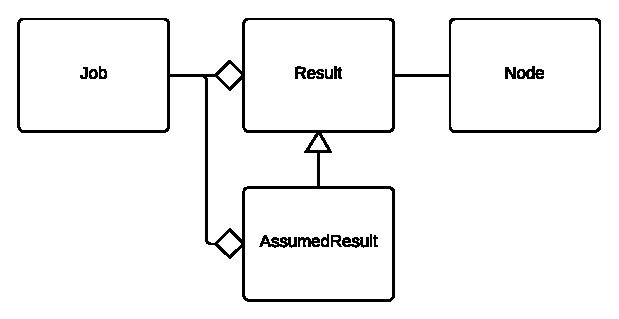
\includegraphics{diagrams/SimulatorClassDiagram.pdf}
\caption{Diagram of classes used in the simulator.}
\label{f:simclassdg}
\end{figure}

\section{Simulator loop}

Simulation is done by evaluating each node in a loop. Time is represented by abstract time unit called \emph{tick}. Every iteration of the loop is simulation of network in consecutive time units. In each iteration, every node is evaluated, by doing as follows:
\begin{itemize}
	\item If node is working on idling, continue to the next node.
	\item If not: \begin{itemize}
		\item If node has just finished job, hand out job, recompute job's correctness and participants' trust.
		\item Find a new job for the node. \begin{itemize}
			\item If job is found, calculate \emph{work time}.
			\item If no job is found, set to idle until next tick. 
		\end{itemize}
	\end{itemize}
\end{itemize}

The ticks are being simulated until all jobs are estimated to be complete. Job is complete when a set of results can be found which have the same \emph{hash} and sum of their \emph{correctness} exceeds $1$.

Upon each iteration, we can plot data such as nodes' trust or percent of completed jobs. Simulator uses gnuplot for this task.

\subsubsection{Work time}
\label{s:worktime}

The program simulates "work time" based on node's performance factor and job's difficulty factor. The work time is actually number of ticks that the node has to wait until it sends back the result and gets a new job. We assume that different nodes will get computing work done faster, and jobs may vary in difficulty, and therefore time to complete. All of this is simulated by the simulator software.

Work time is being calculated using following equation:
\begin{equation}
W(N, J) = 1 + 100 * \text{difficulty}(J) * (1 - \text{performance}(N))
\end{equation}
$W(N, J)$ is the work time (in ticks), $N$ is node for which it is calculated, and $J$ is the job.

Work time has a minimum value of 1, and is directly proportional to the difficulty factor of the job, and inversely proportional to node's performance factor. $100$ is used as a constant to scale work time from $1$ to $101$. In simulator, it needs to be a whole number. The fraction is dropped (results of the calculation is casted to an integer).

\section{Implementation}

We want to be able to simulate networks with hundreds of nodes and thousands of jobs. In order to achieve needed performance, appropriate data structures are used. This section will explain how certain performance critical aspects of simulator are implemented and the rationale behind it.

Set is used as a data structure to keep collection of objects. Ordered set can keep unique elements following a specific order. Operations on sets, such as searching for elements and inserting an element, are of logarithmic complexity.

\subsection{Nodes}

The node collection is an ordered set, where the order is determined by \emph{next working tick}. \emph{Next working tick} is the tick when the node state should change. When a node gets job at tick $10$ and the job is calculated to take $5$ ticks, \emph{next working tick} is $15$. At tick $15$ job will be finished, nodes' trust recalculated and node will get new job. There is no need to check on the node in ticks $11$ to $14$.

\begin{figure}
\centering
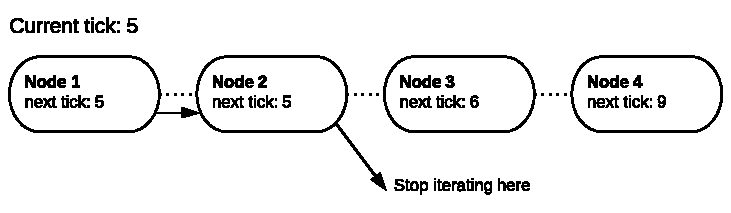
\includegraphics{diagrams/SimulatorNodes.pdf}
\caption{Iterating through simulator nodes. Simulator breaks out of the loop early, skipping nodes that should not be processed in current iteration.}
\label{f:simnodes}
\end{figure}

Because iteration happens on ordered set of nodes, we can stop iterating as soon as we reach node that \emph{next working tick} is higher than current tick. Example of this behavior is shown in figure~\ref{f:simnodes}. The only thing to keep in mind is to reinsert node (to update its position in set and keep set's consistency) when node state is changed and therefore \emph{next working tick} changes.

\subsection{Jobs}

Jobs are kept in ordered set with the order determined by jobs current best correctness, but in reverse. Jobs with highest correctness are first. Because we search a job for nodes very often, it can become performance bottleneck. 

Jobs are selected in a way that node's contribution will get job closer to completion, which is determined by sum of trust of confirmed results of $1$, but also trying not to waste node's computing power. Waste is considered when sum of correctness exceeds $1$ by significant amount. For example, when job's best correctness is $0.8$, there is no reason to give this job again for a node with trust of $0.5$. Node with $0.2$ trust will suffice.

Ordered set of jobs allows us to use bisection to find best matching job. It may happen that the job cannot be given to this particular node, because it already has sent result for it. If so, we start iterating from that node until we find one that we can give to the node.

Failure in finding a job for a node is not an error. The simulator will try again in next tick - state of the network will be changed, and the search may succeed then.

\section{Simulation results}

This section describes experiments performed using the simulator and reason about inner working of the algorithms trying to understand observed behavior.

\subsection{Dishonest nodes}

The first experiment was to measure performance of the network with dishonest nodes. We call dishonest node a node that is randomly sending back incorrect results with probability $P$. The nodes are not colluding with one other, each dishonest node is replying with its own, random, incorrect result, in hopes that it would be accepted by network as a correct one.

We measured average number of results a job needed to have before it was done. The test was performed with different ratio of dishonesty. Figure~\ref{f:confirmations1} shows results of first test. The simulated network had $100$ nodes and $5000$ jobs. Different dishonesty ratios were applied, to all of the nodes, varying from $P = 0.0$ to $P = 0.5$. Dishonesty ratio of $0.0$ means that the node always sends correct results, ratio of $0.5$ means that there is only $50\%$ chance of the node sending correct results. With dishonesty ratio higher than $0.5$, the network was behaving in very erratic way, and very low amount of jobs was being completed.

Average number of confirmations is $\approx 2.15$ when dishonesty ratio is $0$. Reason for this number being higher than $2$ is that the average from the entire project is taken, and when the project starts and trust is not yet established, the number of confirmations is higher.

\begin{figure}
\centering
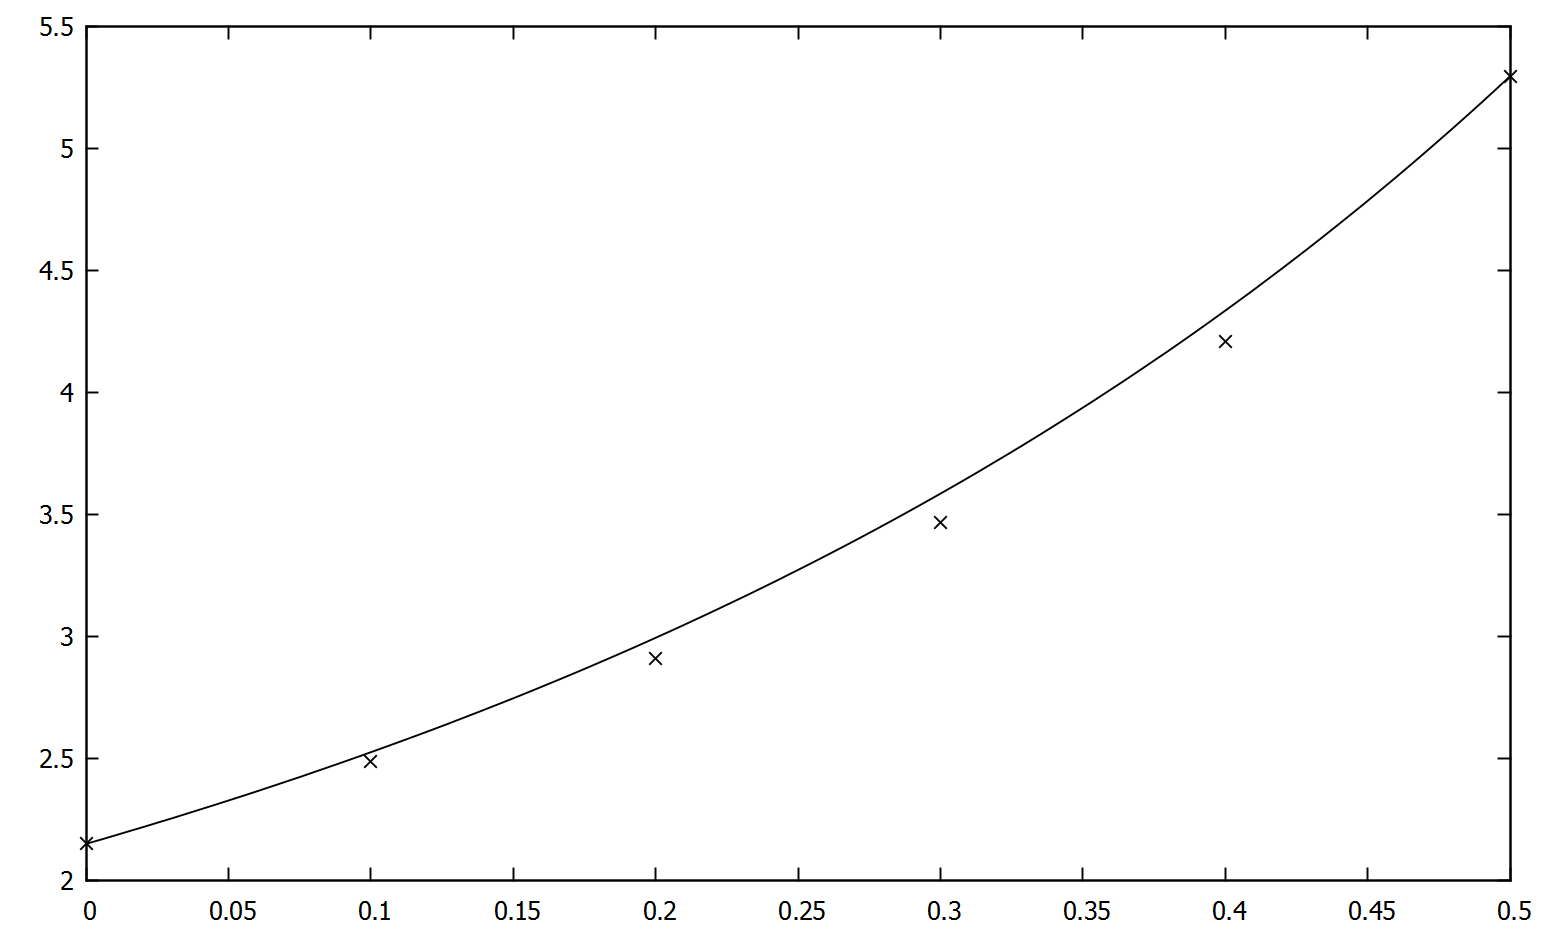
\includegraphics[width=\textwidth]{diagrams/confirmations.png}
\caption{First experiment with dishonest nodes: average number of confirmations (on Y axis) per dishonesty ratio of network (on X axis).}
\label{f:confirmations1}
\end{figure}

Described test simulates environment where the whole network is for some reason inconsistent with results. Another test was performed, that should resemble real life scenario more. In the second test, a part of network has been set to have dishonesty ratio of $0.5$. The rest of it was always honest (ratio of $0.0$). The simulated network also had $100$ nodes and $5000$ jobs. Simulations were performed using different number of dishonest nodes (all with dishonesty ratio of $0.5$). Figure~\ref{f:confirmations2} shows results of the simulation. Network behaves reasonably well even with high number of dishonest nodes. Even when $60\%$ of the nodes send incorrect results, trust model managed to isolate them in a way that network operations were not affected all that much - jobs still needed less than 3 results on average to be confirmed to be correct. For the highest value we tested, $80\%$ of dishonest nodes, the network needed $\approx 4.2$ confirmations on average to mark the job as done.

\begin{figure}
\centering
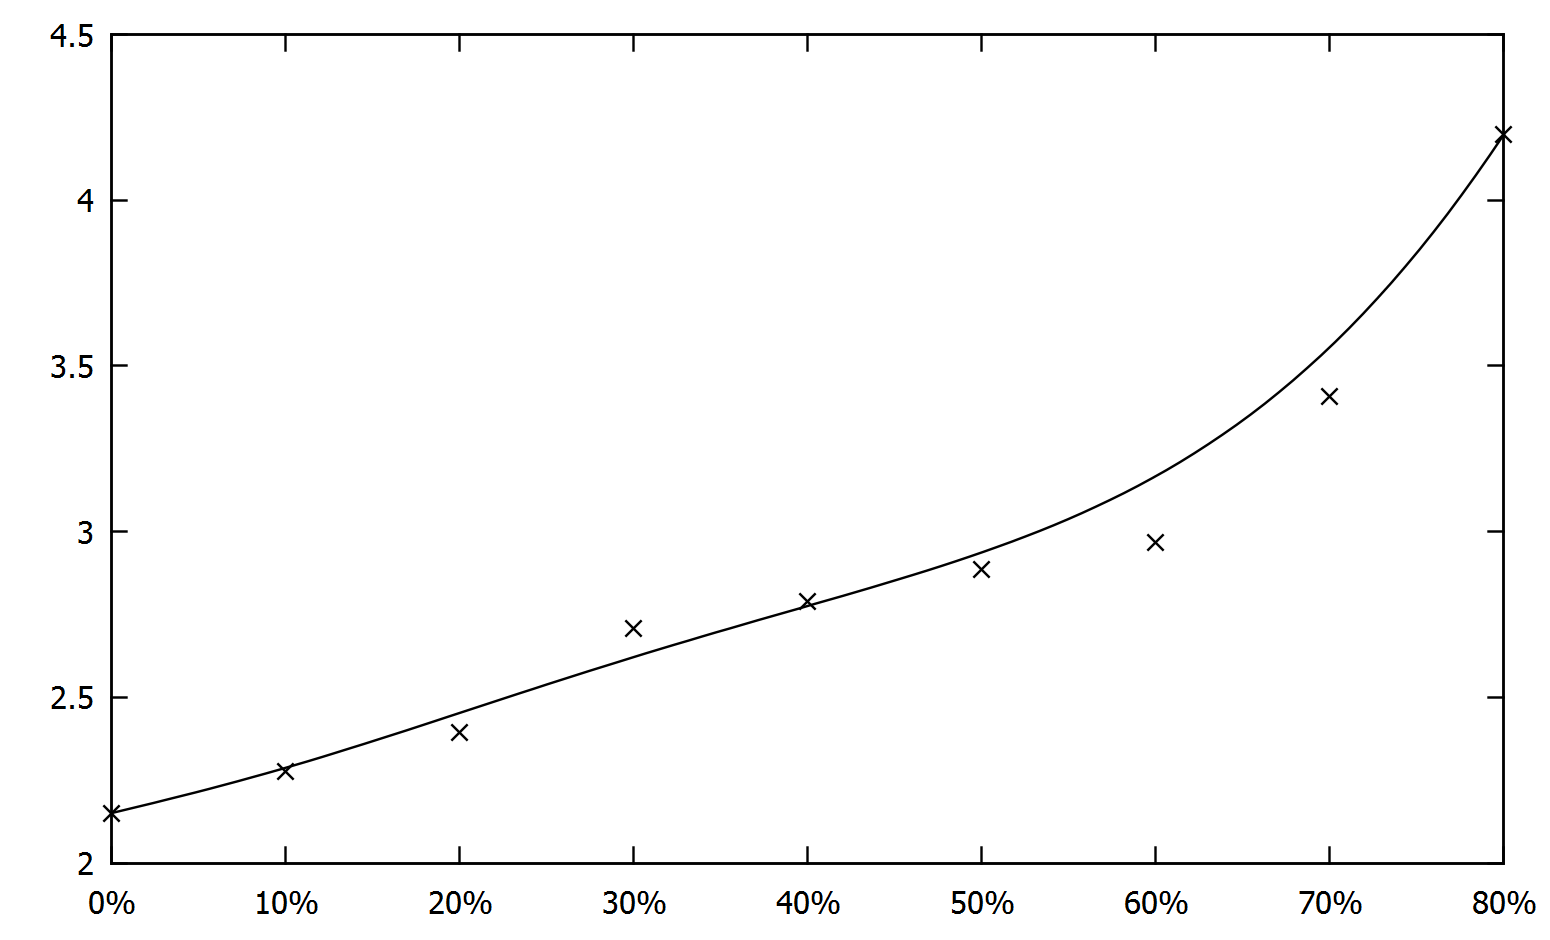
\includegraphics[width=\textwidth]{diagrams/confirmations2.png}
\caption{Second experiment with dishonest nodes: average number of confirmations (on Y axis) per ratio of dishonest nodes (on X axis).}
\label{f:confirmations2}
\end{figure}

Important fact is that all the dishonest nodes were not colluding. When they were to submit an incorrect result, a random one was chosen. For every experiment, no incorrect result was accepted as a correct one. A real life attack on a network would probably consist of many nodes colluding with each other and sending same (but incorrect) results for one problem, which would force the network to accept it as right, if the number of nodes was high enough. Analyzing and defending from such attacks is out of scope of this thesis.

\FloatBarrier

\subsection{Joining and leaving the network}

The next experiment shows change of trust of nodes over time. All simulations have been performed on a network that has $10,000$ jobs and $500$ nodes. All nodes were set to be always honest. Their performance was randomly assigned, as well as job difficulty, which was also random. All nodes have base, constant, trust of $0.1$. Adding a constant trust factor helps the nodes to reach their peak trust faster.

Figure~\ref{f:trust1} shows trust over time of $3$ selected nodes. \emph{Node $2$} is visibly more performant than the other two. We can observe nodes' trust dropping when they are busy computing work, and going back up when they send back the result. The changes are more rapid at the beginning, when nodes still have not performed too much work and slightest change of trust has big effect globally. 

\begin{figure}
\centering
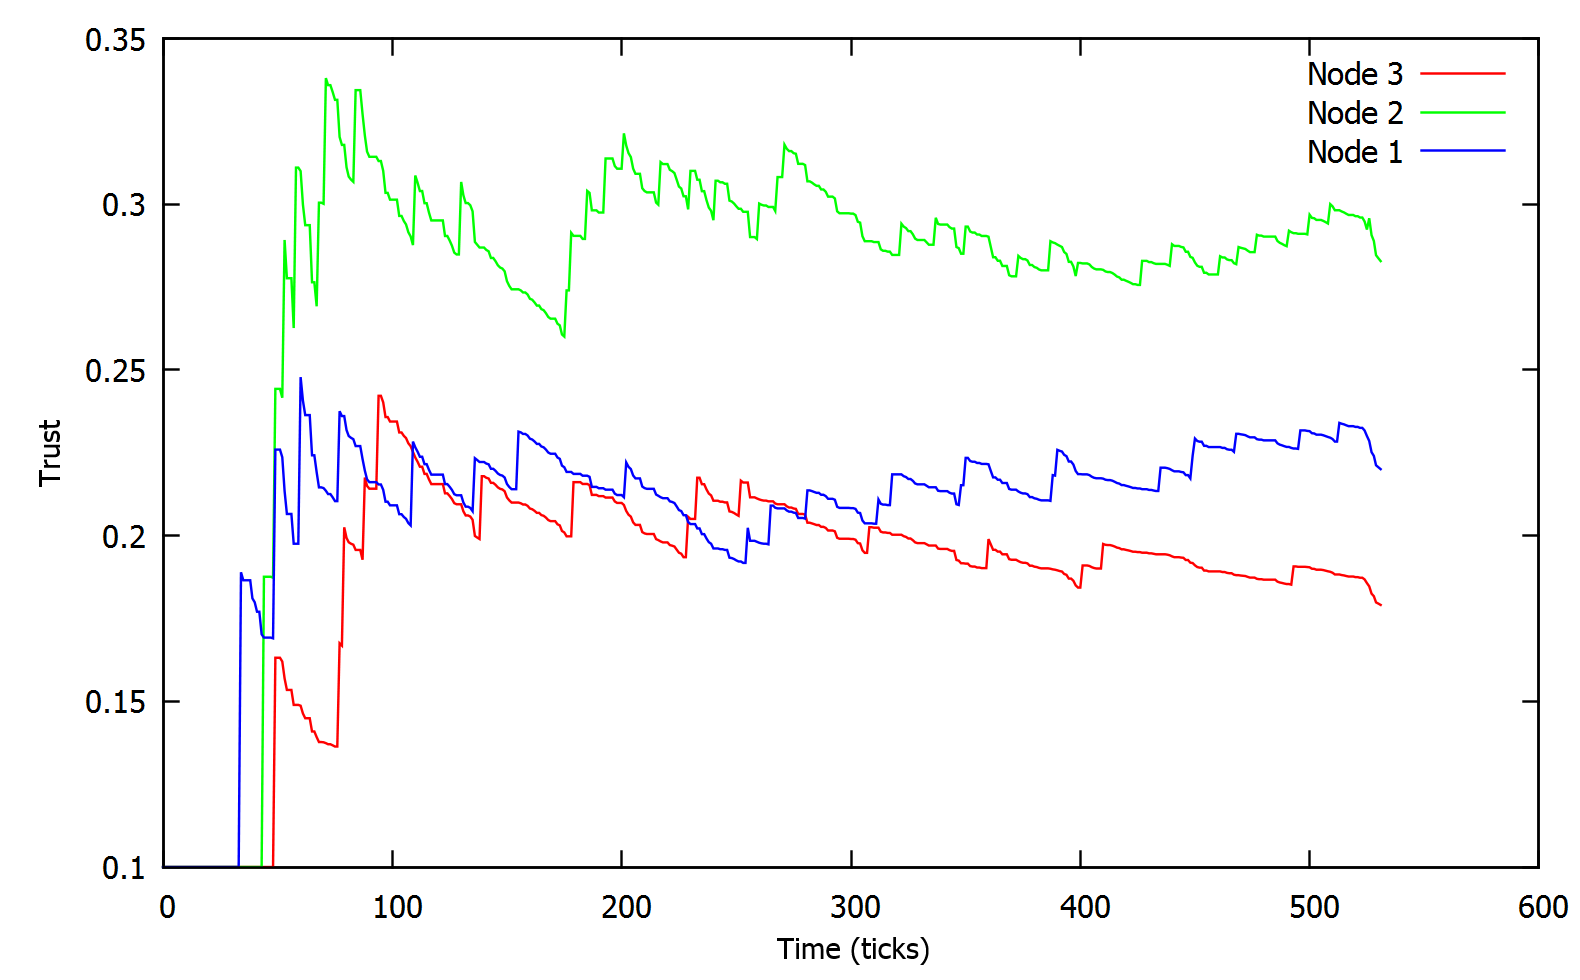
\includegraphics[width=\textwidth]{diagrams/trust1.png}
\caption{Trust of 3 selected nodes during network simulation. Trust is on the Y axis, time (in ticks) on the X axis.}
\label{f:trust1}
\end{figure}

Then, we simulated a network in which one of the nodes joins in the middle of computing project. We can observe its trust quickly growing and reaching its peak, which depends on node's performance factor. Figure~\ref{f:trust_join} shows results of the simulation. \emph{Node 1} is the node joining the project in tick $150$. Shortly after, node sends its first results and its trust raises.

\begin{figure}
\centering
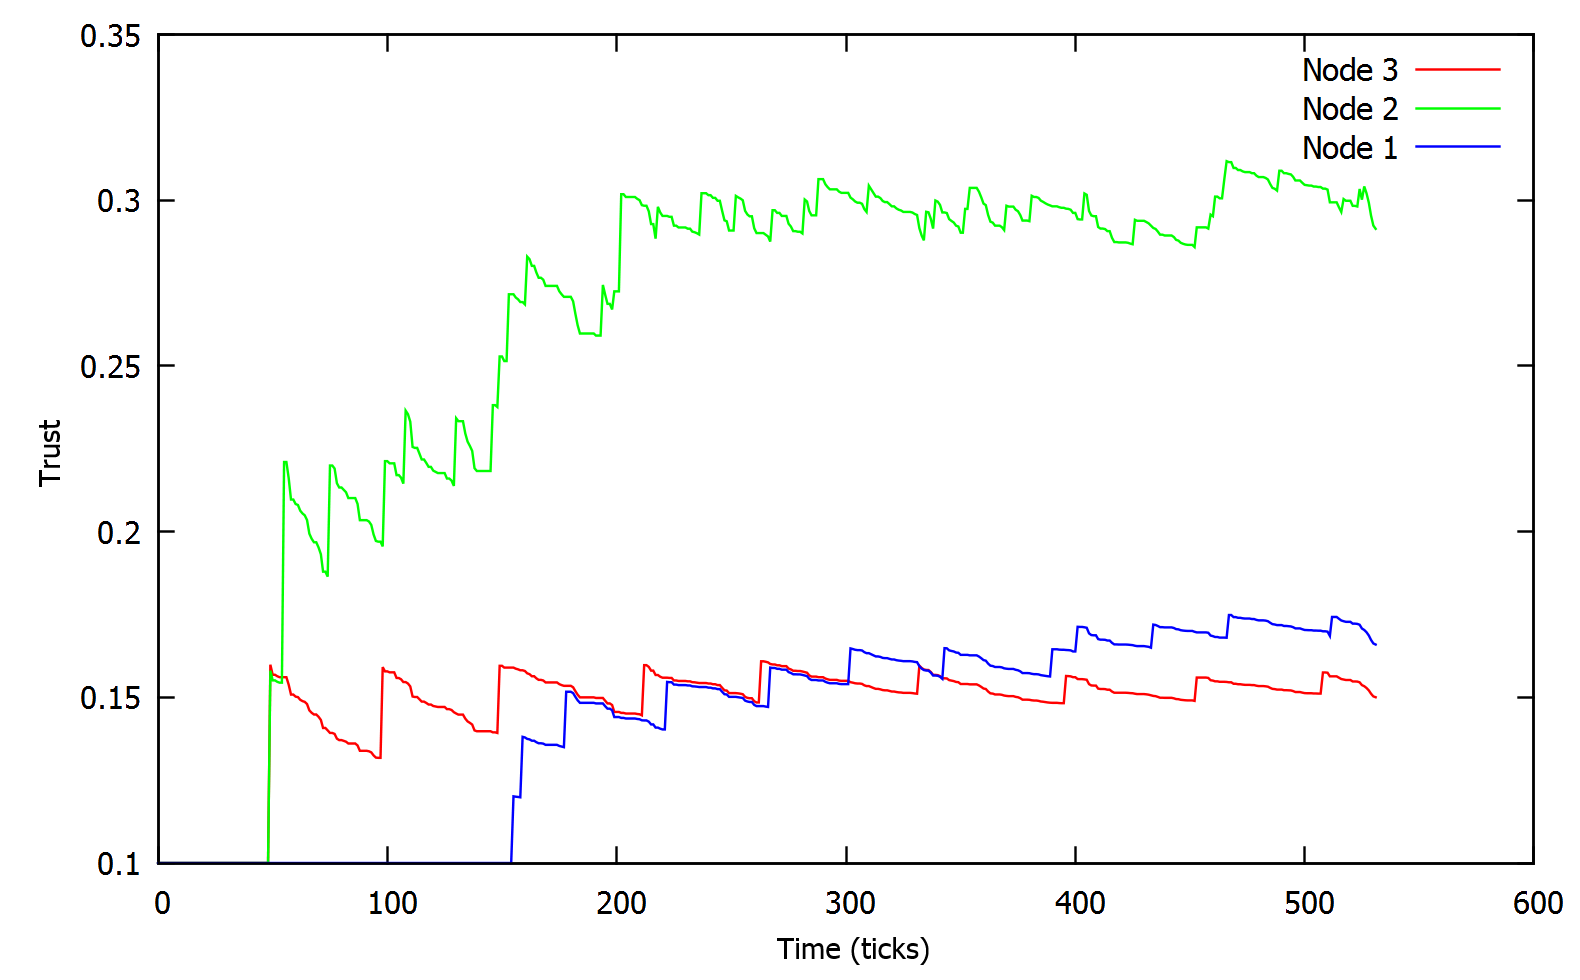
\includegraphics[width=\textwidth]{diagrams/trust_join.png}
\caption{Experiment with node joining the network. Trust is on the Y axis, time (in ticks) on the X axis. In $T_0$ joining node sends its first result and gains trust.}
\label{f:trust_join}
\end{figure}

One simulation was conducted with node leaving the network in the middle of project. Figure~\ref{f:trust_leave} shows the plot of nodes' trust during the simulation. \emph{Node 1} has stopped computing work in tick $250$ and its trust has been getting lower since. Because the project ended around tick $500$, we do not get to observe \emph{Node 1} trust falling all the way to the bottom, but that is what would have happened.

\begin{figure}
\centering
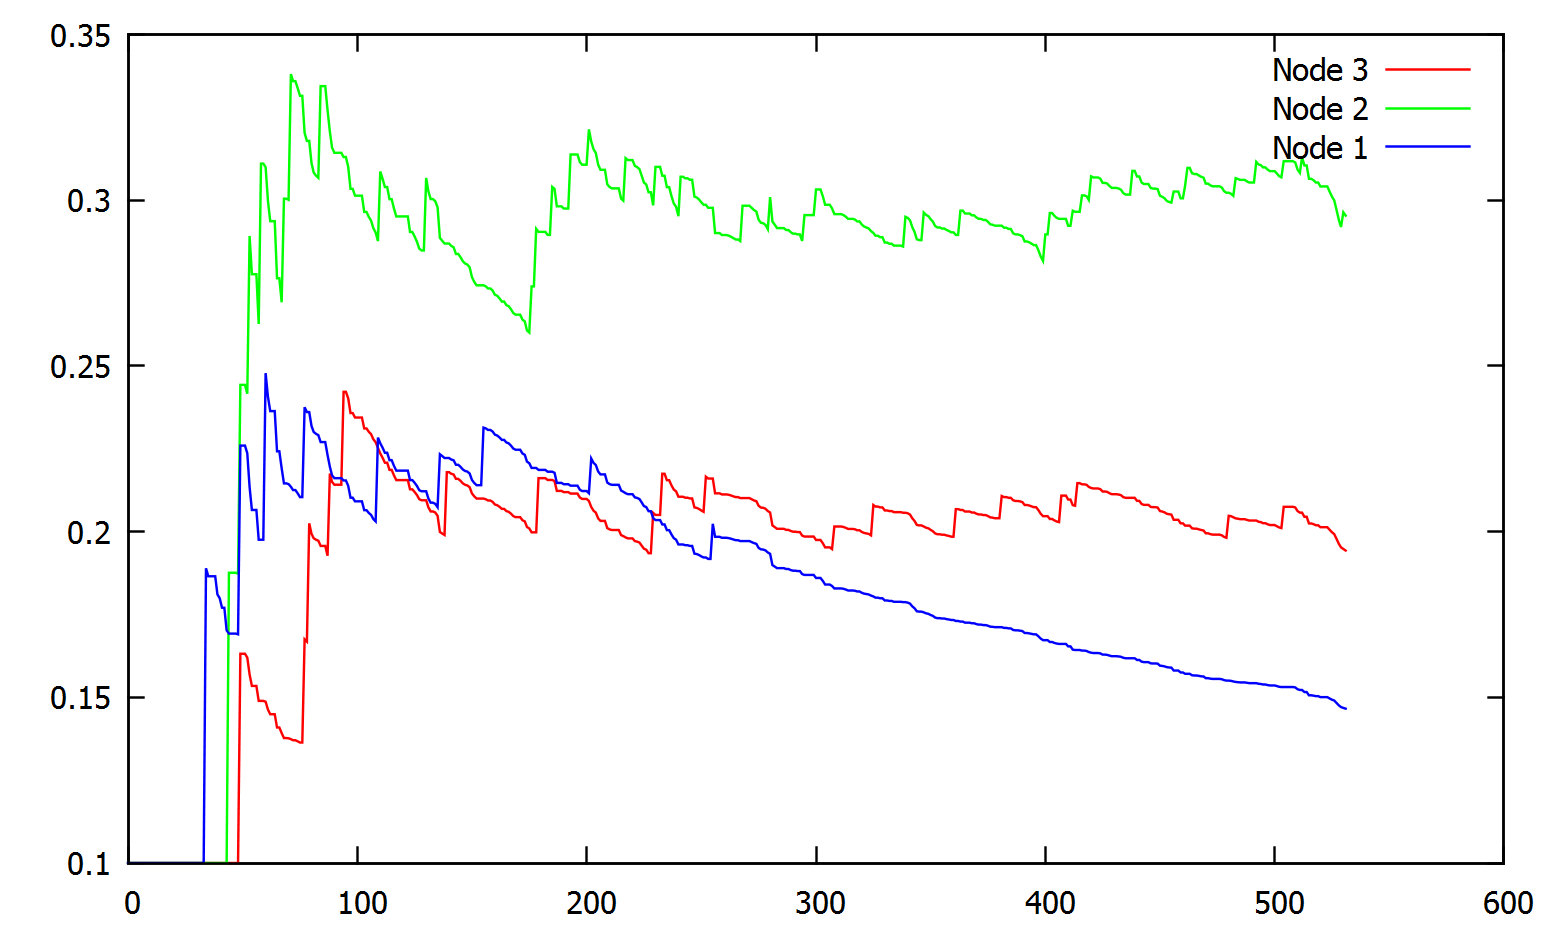
\includegraphics[width=\textwidth]{diagrams/trust_leave.png}
\caption{Experiment with node leaving the network. Trust is on the Y axis, time (in ticks) on the X axis. In $T_0$ leaving node sends its last results and does not do work anymore.}
\label{f:trust_leave}
\end{figure}

\FloatBarrier

\subsection{Special cases}

Next, we tested special cases for the simulation. First one is where there are very few jobs in comparison to the number of nodes. For the simulation, we used a network in which there was only $500$, and $500$ nodes. The results, plotted on figure~\ref{f:less_jobs}, shows that the network can handle such situation as well. The nodes had problem at the beginning to receive jobs (because the competition was high), but it managed to stabilize and the plots look as expected, although in smaller scale - such project was completed very quickly. The average number of sent results per job was $\approx 3.74$. The reason is that the nodes did not get a chance to reach their peak trust.

\begin{figure}
\centering
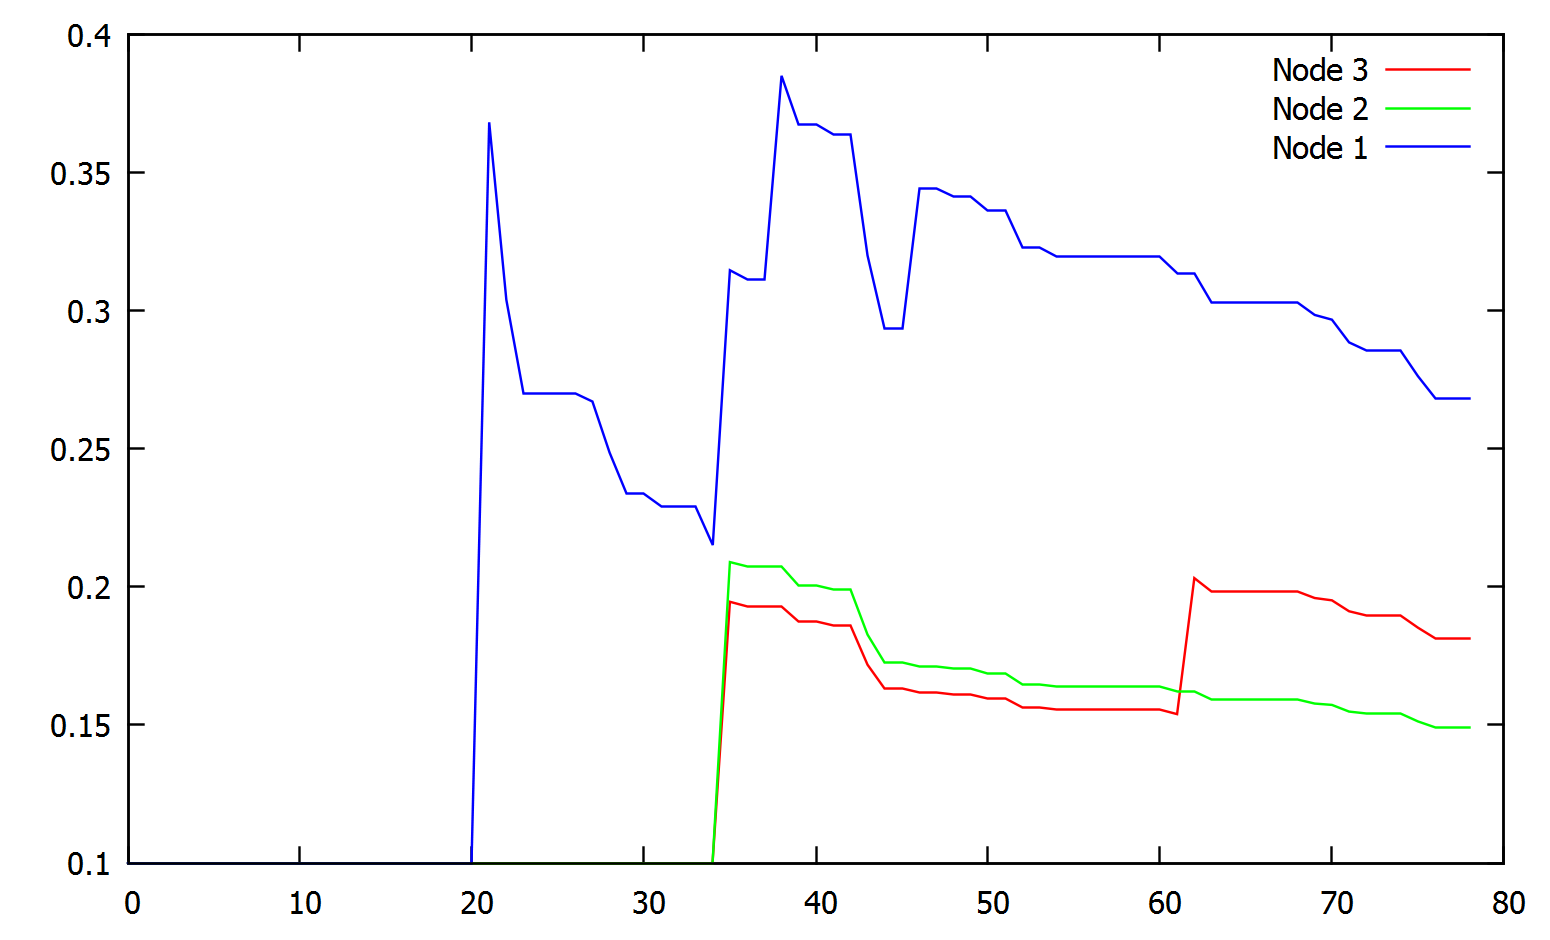
\includegraphics[width=\textwidth]{diagrams/trust_less_jobs.png}
\caption{Experiment where the network had same number of jobs and nodes. Trust is on the Y axis, time (in ticks) on the X axis.}
\label{f:less_jobs}
\end{figure}

Second case is where the network has many jobs but less nodes. The simulation was run with $5000$ jobs but only $50$ nodes. Resulting plot is on figure~\ref{f:more_jobs}. The stabilization phase is longer at first, but then the network behaves normally. It reaches $\approx 2.08$ results per completed job, which is the lowest number achieved in the simulations. This means, that generally it is healthier for the network to have higher number of jobs per node. The network took long to finish the project, but that was expected with amount of nodes this little for project that big.

\begin{figure}
\centering
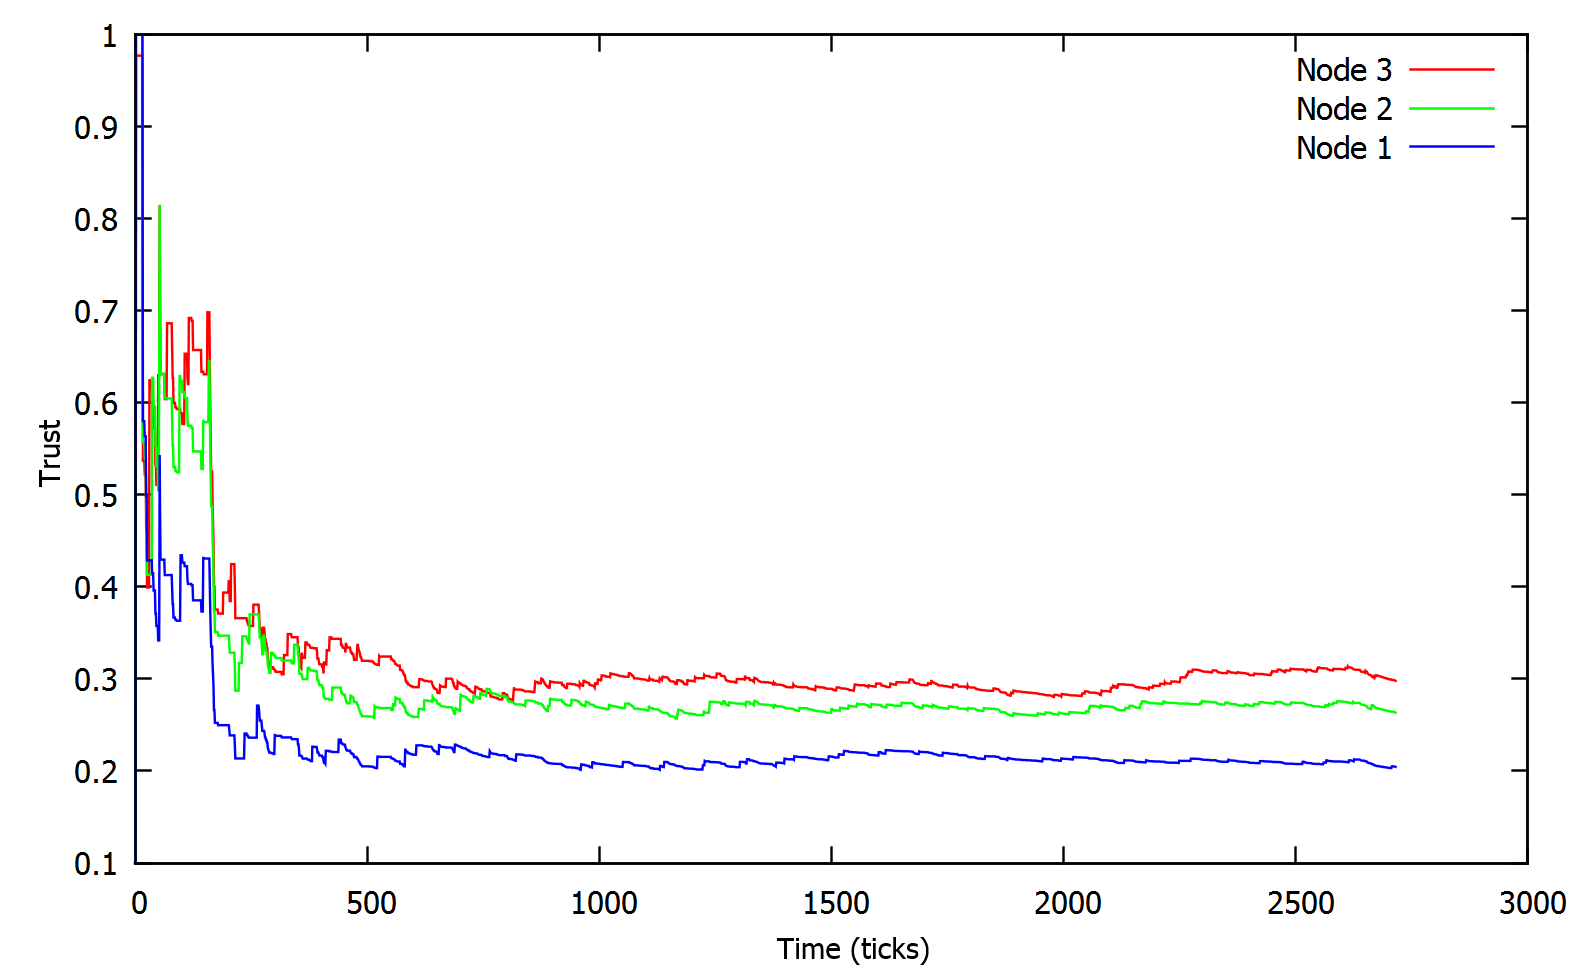
\includegraphics[width=\textwidth]{diagrams/trust_less_nodes.png}
\caption{Experiment with low number of nodes. Trust is on the Y axis, time (in ticks) on the X axis.}
\label{f:more_jobs}
\end{figure}

\FloatBarrier

\subsection{Case of homogeneous network}

In all previous cases, the nodes performance was not distributed evenly across the nodes. This case shows a network where all nodes have the same performance. Results are plotted on figure~\ref{f:evenly}. The project had $10,000$ nodes and $1000$ jobs. We can observe that competition was very high and all nodes had very high trust, approaching $1$.

The network still worked and managed to complete the project. The average number of results per job was $\approx 2.19$. Although this is not a normal case for volunteer networks, it is not uncommon with computing grids, where all of the hardware is similar or even the same. This experiment shows that the developed trust model is applicable to the networks of homogeneous hardware.

\begin{figure}
\centering
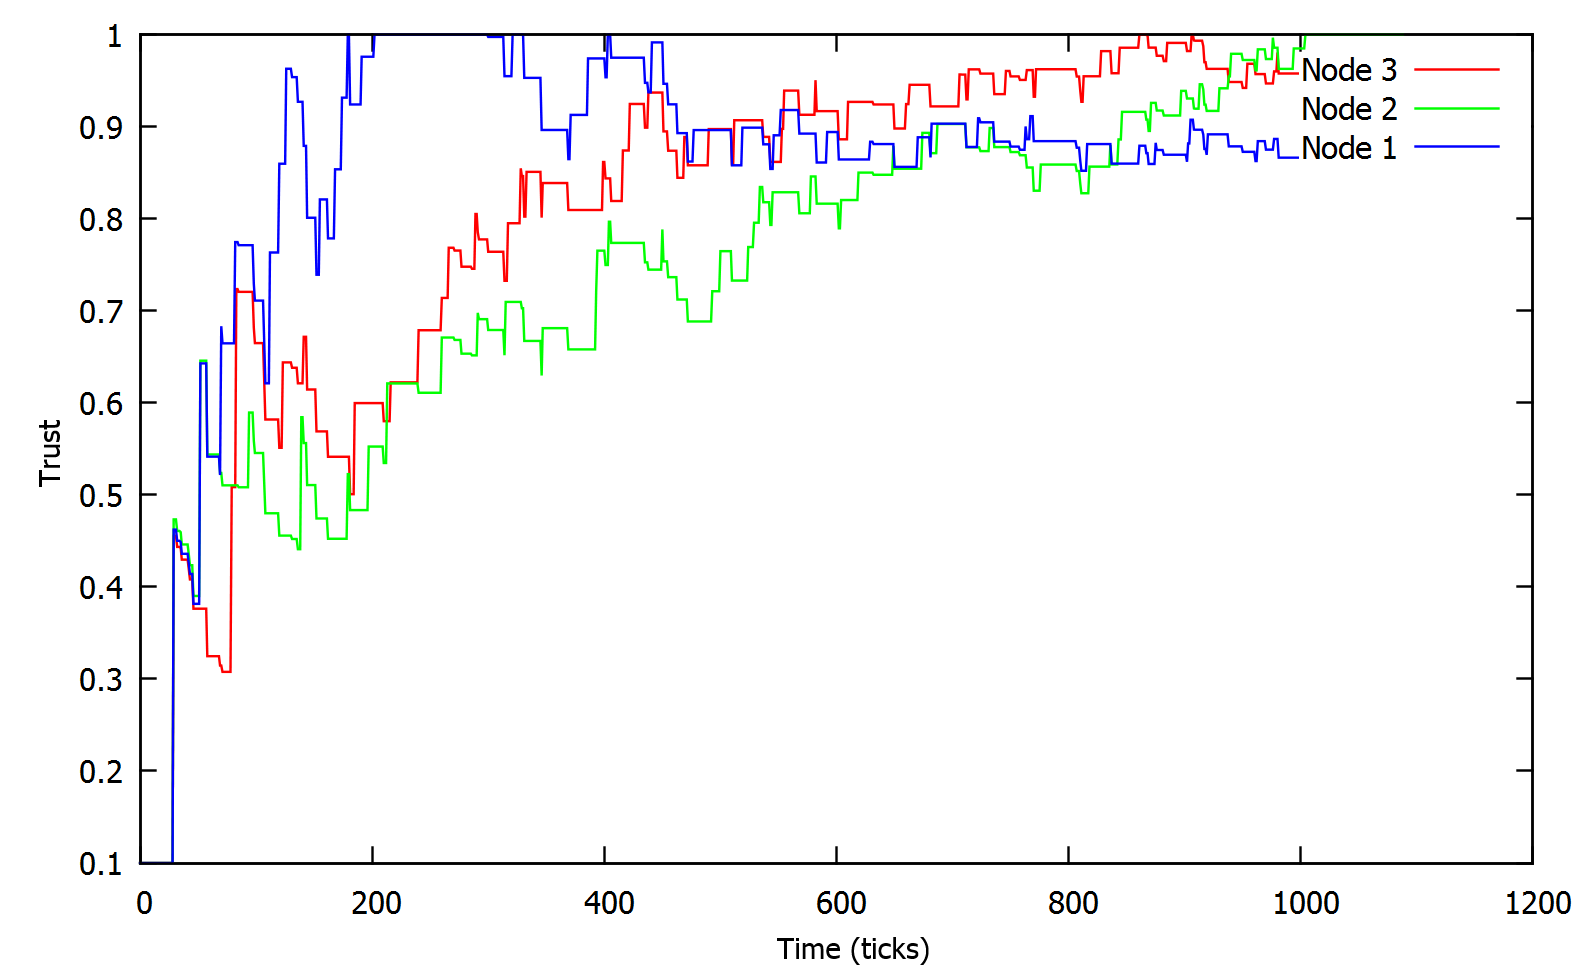
\includegraphics[width=\textwidth]{diagrams/trust_static.png}
\caption{Experiment with network of homogeneous performance. Trust is on the Y axis, time (in ticks) on the X axis.}
\label{f:evenly}
\end{figure}

\chapter{Prototype}
\label{ch:prototype}

This chapter will describe implementation of the prototype, and reason for used technologies.

Prototype was created to test if virtual machine technologies are suitable for use in computing platform. HTTP is leveraged as a communication protocol between nodes and the market. BitTorrent protocol is used to distribute said virtual machines to client. Nodes run VirtualBox virtualization software.

Hypothetical network using system described in this thesis is shown in diagram~\ref{f:protomain}. All nodes connect to the server using HTTP, and communicate with one another using BitTorrent~\cite{cohen2008bittorrent} protocol.

\begin{figure}
\centering
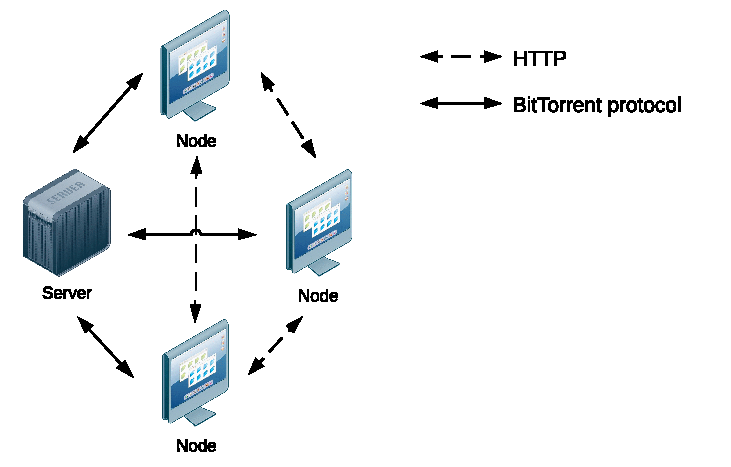
\includegraphics{diagrams/PrototypeMain.pdf}
\caption{Prototype diagram}
\label{f:protomain}
\end{figure}

The prototype implements both client software and the market software, as well as one testing project.

Function specification, that is, the requirements of the prototype, are described in section~\ref{s:funcspec}. Notable implementation details are presented in section~\ref{s:impldet}.

\section{Functional specification}
\label{s:funcspec}

This section presents functional specification of the prototype. It describes responsibilities of both the client and the server software. Communication between them is described, which is done through the \emph{Market API}, as well as method of authentication.

Both server and the client are running in daemon mode, that is, there is no user interface available. User can inspect operation of both programs by looking at the log files. The configuration is being done by editing configuration files with a text editor.

\subsection{Server}

Server is ran by market operator. Server tasks are as follows:

\begin{enumerate}
	\item \label{ps:register} let nodes register themselves,
	\item \label{ps:hand} hand out jobs,
	\item \label{ps:collect} collect results,
	\item \label{ps:measure} measure trust,
	\item \label{ps:track} keep track of project progress.
\end{enumerate}

Task~\ref{ps:register} refers to ability of server to register new nodes and authenticate already registered ones. Node authentication is done with public-key cryptography. Worker uses public/private key pair to to authenticate its request to the server. When connecting for the first time, a permanent record is left in the server's database which is used to recognize that particular client from then on.

"Hand out jobs" task (\ref{ps:hand}) means that server should keep a database of jobs and be able to distribute them to nodes. System presented by this thesis works in a way that the nodes ask for jobs, and the server searches database for suitable job, based on node's trust.

Server should be able to collect results (\ref{ps:collect}) and keep them in a database. By being able to match results with one another and thus confirming them, server is measuring trust (\ref{ps:measure}) of nodes. Those two altogether give the server an ability to decide whether a job is considered finished or not, so the server is able to measure progress (\ref{ps:track}) of the project.

\subsection{Client}

Client is software running on worker computers. Client should be able to:
\begin{enumerate}
	\item \label{cs:auth} authenticate itself to the server,
	\item \label{cs:recv} receive job from the server,
	\item \label{cs:compute} compute received work,
	\item \label{cs:send} send back results of the computation.
\end{enumerate}

(\ref{cs:auth}) means that the client should be able to present itself to the server so both the client can ensure it communicates with entity it think it does, and the server can ensure the client is who it says it is. Methods of doing so are described in section~\ref{s:authentication}.

Receiving jobs from the server (\ref{cs:recv}) consists of two tasks. First is receiving the project, which is the virtual machine and its metadata, from the server. Project files are distributed using BitTorrent technology. After installing and setting the virtual machine up, the client will then ask for job files. Job files are distributed using HTTPS.

When the virtual machine is ready and powered up, job files are sent to the machine and it can start the computation (\ref{cs:compute}). When results are ready, virtual machine sends the results to the client, which then sends them back to the server (\ref{cs:send}).

This process is then repeated. The client asks for next job after finishing one. When there are no jobs left, the client will ask for next project.

The process is also shown in the figure~\ref{f:clientflow}.

\begin{figure}
\centering
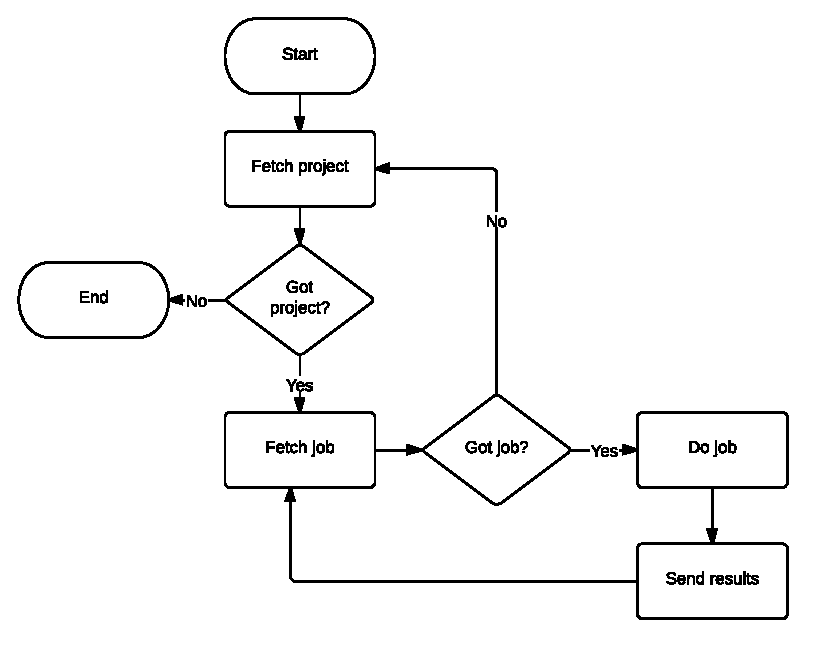
\includegraphics{diagrams/ClientFlowchart.pdf}
\caption{Client flowchart}
\label{f:clientflow}
\end{figure}

\subsection{Authentication}
\label{s:authentication}

Authentication is a two step process. Firstly, the server has to gain trust of the client. The server can do it by either presenting a certificate signed by Certificate Authority, or presenting a self-signed certificate, but transferring the certificate in secure and trusted manner beforehand. For this prototype, we will be working with self-signed certificates, but using the CA is also an implemented option.

Secondly, the server is configured in a way that it will request certificates from the clients. Each client has to generate a key pair and use the private key to authenticate itself when connecting to the server. The certificate fingerprint is used to identify clients. Each client will have different, generated by themselves, key pair, therefore different certificate fingerprint, and due to that, the server is able to identify clients unambiguously using their certificate fingerprints alone.

\section{Architecture}

This section shows how the application is organized. Code for both server and client is separated into modules, using Node.js module system\footnote{Module system is described further in Node.js documentation \url{http://nodejs.org/api/modules.html}}.

Responsibilities of each module will be discussed, and some more significant parts are going to be presented in detail.

Architecture is presented on the figure~\ref{f:arch}. Then, each module's responsibilities are briefly described.

\begin{figure}
\centering
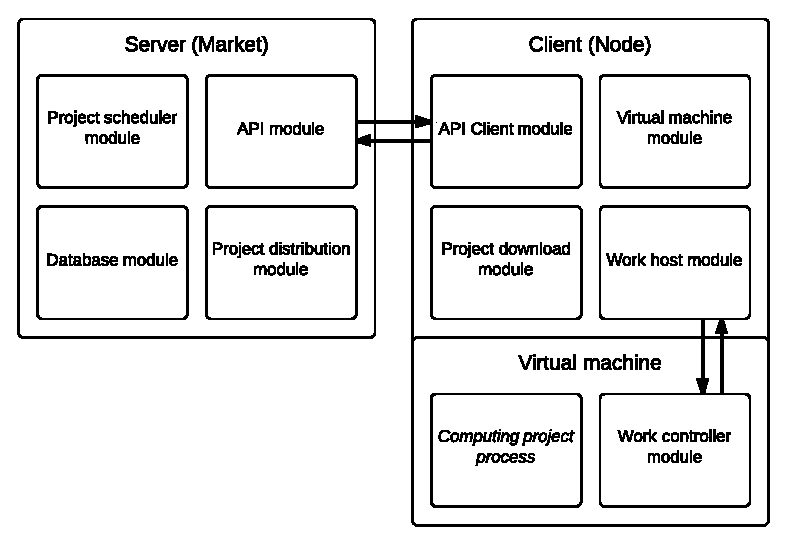
\includegraphics{diagrams/Architecture.pdf}
\caption{Architecture of the prototype. 3 environments can be distinguished: \emph{Server}, \emph{Client}, and \emph{Virtual machine}. Communication between those has been marked with arrows. Only modules with an outgoing arrow can communicate across boundaries of their environments.}
\label{f:arch}
\end{figure}

\subsection{Client}

This section describes modules visible in client environment, pictured on figure~\ref{f:arch}.

\begin{description}

\item[API module] implements very thin client for calling methods exposed by the server. The methods, as well as their purposes, are described in section~\ref{s:cliapi}.

\item[Project download module] is used to fetch project data (virtual machine image and metadata). Internally it uses BitTorrent technology to do that, which allows not only direct transfer from the server, but also peer to peer transfer from other nodes.

\item[Virtual machine module] is used to control virtual machines. VirtualBox\footnote{Virtualbox is a free virtualization product by Oracle, \url{https://www.virtualbox.org/}.} is used as a virtualization engine. This module is used to set up and start virtual machines, when the client starts working on a project.

\item[Work host module] is used to communicate with computing program that is running withing the virtual machine. Because we generally do not place restrictions on what computing programs can be used, special layer has been created in order to exchange data and results with programs. \textbf{Work host module} communicates with \textbf{Work controller module} which is running in virtual machine, and can directly 

\end{description}

\subsection{Server}

This section describes modules visible in server environment, pictured on figure~\ref{f:arch}.

\begin{description}

\item[API module] is used to host an the API for the clients to use. HTTPS is used as the method of communication. Methods implemented within this module are not used internally by server, they are called by the clients instead.

\item[Project scheduler module] is responsible for assigning workers to project and distributing jobs among workers withing a project. For this prototype, assigning to project is done using very simple method. Project scheduler chooses the first project that has undone jobs. Distributing jobs is done using an implementation of algorithm described in section~\ref{s:jobdist}.

\item[Database module] serves as a layer between CouchDB database and the server program.

\item[Project distribution module] is responsible for distributing project files (virtual machines and their metadata). This module prepares a \emph{.torrent} file to return to client. It also starts its own BitTorrent tracker and serves initial (called the \emph{seed}) download.

\end{description}

\section{Market API}
\label{s:cliapi}

This module provides a way for clients to communicate with the server. The communication happens over HTTPS, with use of authentication described in section~\ref{s:authentication}. The module follows REST\footnote{\emph{Representational state transfer}, model for how to build services.} guidelines on how to implement an API.

Client API exposes the following methods that can be remotely called by clients:

\subsection{fetchProject}

\emph{fetchProject} API method is used by clients to discover on what project there will be working on. Result of that call is project id, that will be used internally to fetch project data (distributing projects is explained further in section~\ref{s:torrent_dist}).

This call will result in assigning client to a project when the client is not already in a project. Otherwise, current project id is returned, and no changes are made to the client. So this call is not only used to request the project, but also to discover what project is the client working on, after it starts.

\subsection{fetchJob}

\emph{fetchJob} method is used to discover what job client will be working on. Result of this call is job id, which is used later to fetch job data, and to send results back (with \emph{sendResult} method).

This call results in finding new work for client only when client has finished previous job (or has not fetched a job in their project yet). There is no way of changing job or aborting one. When client already has a job and calls \emph{fetchJob}, job id of current job is returned, and no changes are made to the client. \emph{fetchJob} is used when client starts (along with \emph{fetchProject}) to start working, whether it will result in getting new project or new job (or both), or continuing where the client has left.

\subsection{sendResult}

\emph{sendResult} is called by client when their computation is finished and results are ready to be sent back. Results are sent as a binary data and the server does not care about the format. This is done to ensure maximum flexibility as far as projects are concerned. After receiving, initial correctness of the is computed, which is the reliability of the node. 

Hash of the data (using SHA1) is computed. We can now easily compare newly received result to results that have been handed in before. For each of the results that are equal (hash values match), \emph{total score} is increased. Job record keep \emph{total score} for each unique result received, by mapping it to the hash value. When unique result's score exceeds $1$, the job is marked as \emph{done}.

If there is are no prior results with hash matching, the raw data is also saved to the database.

Example of completing results is shown in figure~\ref{f:sendresultsex}.

After sending the result, client should ask for another job, using \emph{fetchJob} method.

\begin{figure}
\centering
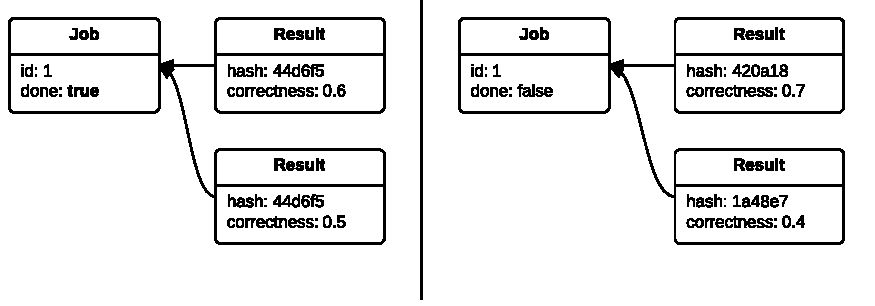
\includegraphics{diagrams/SendResultsExample.pdf}
\caption{Two examples of job with two results. Job in example on the left is marked as \emph{done}, because sum of correctness of results exceeds $1$. Example on the right shows undone job, because even though correctness exceeds $1$, the nodes has not agreed on the results (the hash differs).}
\label{f:sendresultsex}
\end{figure}

\section{Implementation details}
\label{s:impldet}

\subsection{Distribution and download modules}
\label{s:torrent_dist}

\emph{Distribution module} on the server, and corresponding \emph{download module} on the client, are used to to effectively transfer project files (stored on the server) to the client. BitTorrent protocol is used to save bandwidth and speed up the transfer.

\emph{node-torrent}\footnote{https://github.com/zapu/node-torrent} library is used by both modules. It is used to parse \emph{.torrent} files. \emph{node-torrent} is also a BitTorrent client. Important fact is that the server also runs a BitTorrent client and takes part in BitTorrent data exchange. In theory, after the first worker of the project downloads the project data, server could stop serving it. But in practice, it is better for the network if the server remains active.

Download module uses \emph{node-torrent} module to provide ability to use BitTorrent protocol to fetch project data. Project data consists of VirtualBox virtual machine files. The module export one function, which given the \emph{.torrent} file, will proceed with the download and call back when it is completed.

The \emph{.torrent} contains all the metadata necessary to download and verify data, which in our case is virtual machine image. Also included are URL addresses of torrent trackers, which serve as a "meeting point" for nodes, in case node discovery via Distributed Hash Table fails.

Figure~\ref{f:clientprojdownload}~shows how all three modules (\emph{Market API}, \emph{Download module}, and \emph{Virtual machine module}) are used to fetch virtual machine with project data from Market. First an API call is made to acquire \emph{.torrent} file. Then, \emph{Download module} is used to connect to peers and fetch torrent data to local file system. The \emph{virtual machine module} then registers the downloaded virtual machine. This action makes it ready to use.

\begin{figure}
\centering
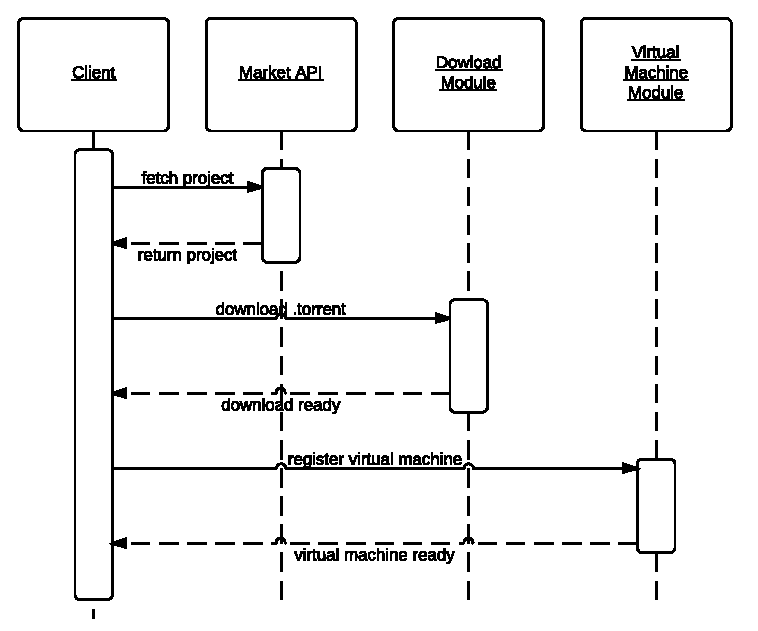
\includegraphics{diagrams/ClientProjectDownload.pdf}
\caption{Sequence diagram showing how virtual machine is fetched from Market and then registered within Virtual machine module (described in section~\ref{s:c_vm_mod}).}
\label{f:clientprojdownload}
\end{figure}

\subsection{Virtual machine module}

\label{s:c_vm_mod}

\begin{comment}
http://www.virtualbox.org/manual/ch08.html
\end{comment}

Virtual machine module is used to launch the project virtual machine using VirtualBox virtualizer. Internally, it uses \emph{VBoxManage}\footnote{VBoxManage is an utility provided by Virtual Box. \url{http://www.virtualbox.org/manual/ch08.html}} for operating on Virtual Box. \emph{VBoxManage} provides functionality, such as

\begin{description}
\item[list] to list virtual machines,
\item[import] to import virtual machine file,
\item[unregistervm] to remove already added virtual machine,
\item[controlvm] to power off or reset virtual machine,
\item[startvm] to start virtual machine.
\end{description}

The module is mostly a wrapper over \emph{VBoxManage} command line utility. The following are code listings\footnote{Consult \url{http://maxtaco.github.io/coffee-script/} website for syntax reference.} for implementations of the \emph{list} wrapper and \emph{import} wrapper. \emph{list} wrapper not only calls \emph{VBoxManage}, but also parses the output to produce JavaScript array of objects, instead of flat text.

\begin{lstlisting}[caption=Function wrapping \emph{vm list} method.]
vm_list = (what, autocb) ->
  await exec "#{$.VBoxManage} list #{what}", 
    defer error, stdout, stderr

  throw error if error

  results = []

  for line in stdout.split("\n")
    matches = line.match /"(.*)" \{([0-9a-f\-]*)\}/
    if matches?
      results.push 
        name: matches[1]
        guid: matches[2]

    return results
\end{lstlisting}

\begin{lstlisting}[caption=Function wrapping \emph{vm import} method.]
import_vm = (path, name, autocb) ->
  await exec "#{$.VBoxManage} import #{path} --vsys 0 --vmname #{name}",
    defer error, stdout, stderr

  throw error if error
\end{lstlisting}

\subsection{Work module}
\label{s:workmod}

Work module is used to communicate with project executable running within virtual machine. It works by creating a HTTP server in local network (network between the virtual machine and the host operating system). The project then makes requests to this web server, receiving work items, until there is no more work left. Sequence diagram in figure~\ref{f:clientseq} shows an example situation where work is fetched from the market (\emph{MarketAPI}), a virtual machine is powered on (via \emph{VM Module}) and data is exchanged with computing program on the virtual machine using \emph{work module} (\emph{Virtual machine project} on the diagram).

\begin{figure}
\centering
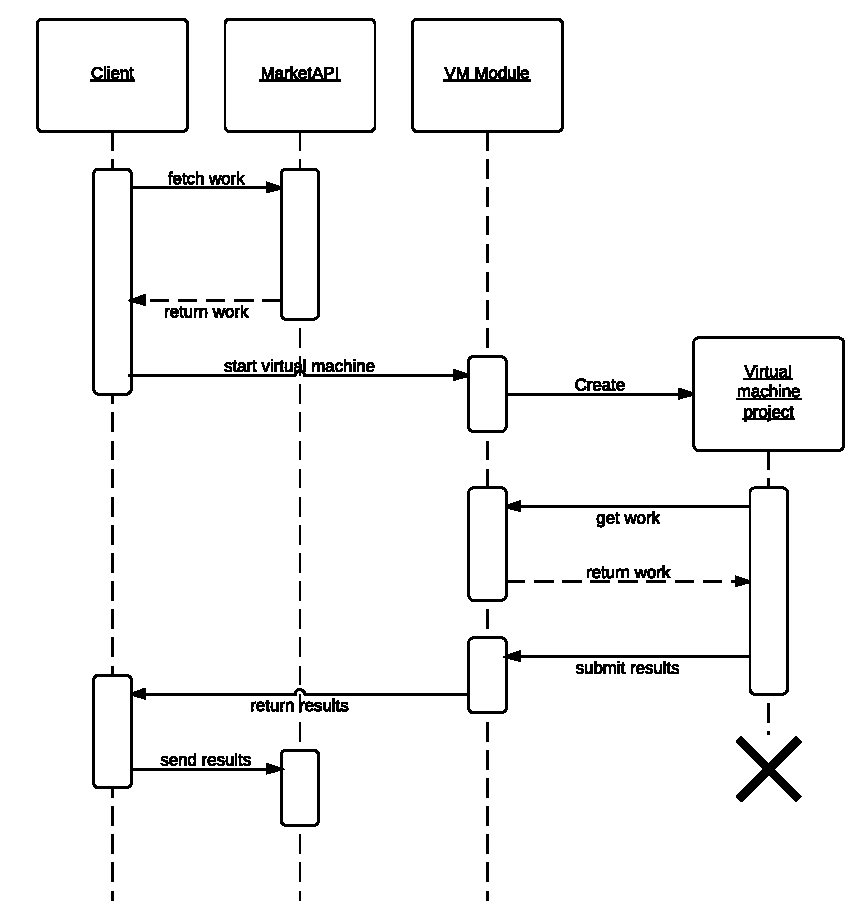
\includegraphics{diagrams/ClientSequence.pdf}
\caption{Sequence diagram showing interaction between client, Market module, Virtual machine module and Work module.}
\label{f:clientseq}
\end{figure}

The protocol is based on HTTP and uses simple GET and POST methods. First, the guest OS is able to ask for job data when it is done setting itself up, using GET request. Then, after computation finishes, it does a POST request to send job computation results. It is important to note that the communication is one-sided as far as data exchange is considered - guest OS initiates both transferring job data and transferring job results. The protocol, however, describes one action in which the host OS initiates communication.

\subsection{Database}

CouchDB\footnote{http://couchdb.apache.org/} is used as database engine. CouchDB is an open source NoSQL database that uses JSON\footnote{Javascript Object Notation, http://www.json.org/} documents. It also allows storing files. Ability to store binary data and the fact that it operates on Javascript Objects made it feasible to use this database engine in the prototype.

Prototype uses \emph{cradle}\footnote{https://github.com/flatiron/cradle} Node.js library to connect to CouchDB.

In the prototype, we use two types of documents. One for projects and one for jobs.

\subsubsection{Project documents}

Example project document looks as follows:

\begin{lstlisting}[caption=Project document in JSON format.]
{
   "_id": "737c253d85f094381717159a55007268",
   "type": "project",
   "participants": [
       "a26ef8e8165be078e324f62629575c37f69f2d83",
       "d0efb2a9fd86ef76822f72ad245e0565ed299263",
   ],
   "_attachments": {
       ...
   }
}
\end{lstlisting}

\begin{description}
\item[\_id] is an internal CouchDB field, which is an unique id of the document.
\item[type] is always set to "project", defines document type.
\item[participants] is the list of all nodes participating in the project. Each node is represented by hash of its public key. For more information about using keys for this, refer to section~\ref{s:authentication}.
\item[\_attachments] is internal CouchDB field for attachment. Each \emph{project} document has one attachment called "program", in which virtual machine image is stored.
\end{description}

\subsubsection{Job document}

Example job document looks as follows:

\begin{lstlisting}[caption=Job document in JSON format.]
{
   "_id": "737c253d85f094381717159a55007cfa",
   "type": "job",
   "project_id": "737c253d85f094381717159a55007268",
   "results": [
       {
           "node": "a26ef8e8165be078e324f62629575c37f69f2d83",
           "score": 0.006756688654422763,
           "hash": "1fb021c0a2a953d76a20f064f4a0b8ec6e307687"
       },
       {
           "node": "d0efb2a9fd86ef76822f72ad245e0565ed299263",
           "score": 0.19533568197607692,
           "hash": "1fb021c0a2a953d76a20f064f4a0b8ec6e307687"
       }
   ],
   "requests": [
   ],
   "_attachments": {
       ...
   }
}
\end{lstlisting}

\begin{description}
\item[\_id] is an internal CouchDB field, which is an unique id of the document.
\item[type] is always set to "job".
\item[results] is array of result objects. Each object has following notation:
  \begin{description}
  \item[node] is the id of node sending the result.
  \item[score] is correctness of node when sending the result.
  \item[hash] is result of hash function applied to result data. It is used to compare the results (if their hash matches, we assume the results are identical).
  \end{description}
 \item[requests] is an array that holds ids of nodes that has been sent the job and the market is awaiting their results. It is the equivalent of \emph{AssumedResult} from the simulator (\ref{s:simdesign}).
 \item[\_attachments] is the CouchDB field for attachments. Job document contains job data that is sent to clients, and results that are computed by clients and sent back.
\end{description}

Each time a node sends its result, we add an item to \emph{results} array. Then, if no other result exists with the same hash, we also store attachment with result data.

\section{Test project}

The prototype comes with an example computing project. The project runs on Node.js platform and is installed under Arch Linux\footnote{https://www.archlinux.org/}. Virtual machine image for the project is 400MB in size. The project is installed as an init script and it starts as soon as system is up. Program then uses protocol described in section~\ref{s:workmod} (\emph{Work Module}) to acquire job data. Same protocol is used to send the results back.

\subsection{The problem}

The project computes Cunningham chains~\cite{andersen2005cunningham}, which are sequences of prime numbers, that follow that

\begin{equation}
p_i = 2^{i-1}p_1 + (2^{i-1}-1)
\end{equation}

Jobs for the project are simply pairs of numbers, first number \emph{from} to start the search, and the second number where the search should end.

\begin{lstlisting}[caption=Javascript code for searching Cunningham chains.]
checkChain = function(num) {
  if(!isPrime(num))
    return null;

  var list = [ num ];
  var coeff = 2;
  for(;;) {
    var val = coeff * num + coeff - 1;
    if(!isPrime(val)) {
      return list.length > 1 ? list : null;
    }

    coeff *= 2;
    list.push(val);
  }
}

module.exports = function(work) {
  var results = [];
  for(var i = work.from; i <= work.to; i++) {
    var chain = checkChain(i);
    if(chain) {
      results.push(chain);
      console.log("Got chain", chain);
    }
  }
  return results;
}
\end{lstlisting}

\subsection{Test run}

The prototype is ran from the console and informs user about its progress using \emph{standard output}. Right after running the client applications, user sees:

\begin{lstlisting}[caption=Standard output of client application.]
Working on project 59ccf0abd01ab22454c428d78b007a5d
Downloading project virtual machine files...
  downloading [===================] 100% 0.0s

Download complete
Download completed, setting up VM...
Importing VM
Starting VM
\end{lstlisting}

Which shows that client has properly registered in project, managed to download virtual machine and set it up within VirtualBox.

We can inspect that the machine is running by using VirtualBox GUI (shown on image~\ref{f:vboxgui}).

\begin{figure}
\centering
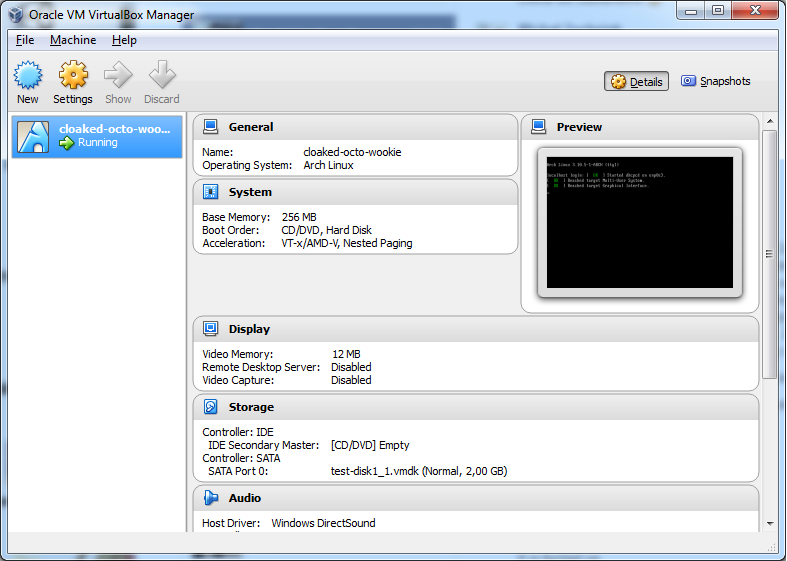
\includegraphics[width=\textwidth]{images/virtualbox.png}
\caption{VirtualBox GUI showing imported and running virtual machine.}
\label{f:vboxgui}
\end{figure}

Then, the client will receive work from the server, send it to the virtual machine, and wait for computation results. This will be repeated until the program is stopped, or there is no more work left for this particular client.

\begin{lstlisting}[caption=Standard output of client application.]
got work 1
Waiting for results...
Submitting work...
Done
...
Done
{ code: 404, body: 'No more work' }
Powering down and removing VM
\end{lstlisting}

We can then inspect, on the server side, results that has been received. In this particular project, results are kept in JSON format, and each result file contains an array of chains, where chain is also an JSON array.

\begin{lstlisting}[caption=Listing of example result file.]
[
  ...
  [394811,789623],
  [395189,790379,1580759,3161519],
  [395201,790403],
  [395261,790523],
  [395273,790547],
  [395303,790607],
  [395849,791699],
  [395891,791783],
  [396239,792479,1584959,3169919],
  ...
]
\end{lstlisting}
\chapter{Conclusions}

The goal of this thesis was to research feasibility of building distributed computing system based on volunteer computing. Such system could be used to create Internet computing markets and potentially reduce needs to employ commercial computing grids, while encouraging both commercial and academic institutions to use distributed computing - because of lowering the costs of using the method. Part of lowering the costs could be the ability to use currently owned hardware and connect it to the system as computing nodes, therefore getting some of the spent money back.

Simulations were performed to see dynamics of volunteer computing system and research algorithms needed to efficiently compute work in a distributed way. Simulations have shown that proposed models can be used to provide a way of collecting and verifying results in a volunteer computing system or a computing cluster. However, defense from coordinated attacks using lots of colluding malicious nodes turned to outside of the scope of this thesis, because it is a huge challenge on its own. Special protections would have to be designed and employed just to protect from such attacks.

Simulations presented in this thesis show a significant improvement over our previous simulator~\cite{zochniakreliable}. Firstly, we were able to simulate networks as big as $500$ nodes and $10,000$ jobs (previously: $50$ nodes and $1,000$ jobs). Secondly, changes in the job distribution model, and the trust model, caused the average number of confirmations to become lower in networks with malicious nodes. Also, the stabilization phase of computing project has been mostly eliminated.

A prototype was created, to investigate technical difficulties of building such system. Prototype proved that use of BitTorrent is feasible way of distributing projects, and that VirtualBox can be used as virtualization technology in order to provide promised flexibility of defining computing projects. 

\section*{Possible improvements}

lorem improvements andasd improvements

\bibliography{praca}{}
\bibliographystyle{plain}

\end{document}